% correct phenotype table in SI
% correct section details in SI
%------------------------------------------
\documentclass[onecolumn,,10pt]{IEEEtran}
\let\labelindent\relax
\usepackage{enumitem}
\usepackage{etex}
\usepackage{amssymb,amsfonts,amsmath,amsthm}
\usepackage{graphicx}
%\usepackage[usenames,x11names, dvipsnames, svgnames]{xcolor}
\usepackage{amsmath,amssymb}
\usepackage{dsfont}
\usepackage{amsfonts}
\usepackage{mathrsfs}
\usepackage{array}
\usepackage{xr}
\usepackage{multirow}
%\usepackage{multirow}    
%\usepackage[T1,euler-digits]{eulervm}
%\usepackage{times}
%\usepackage{pxfonts}
\usepackage{tikz}
\usepackage{pgfplots}
\usetikzlibrary{shapes,calc,shadows,fadings,arrows,decorations.pathreplacing,automata,positioning}
\usetikzlibrary{external}
\usetikzlibrary{decorations.text}
\usepgfplotslibrary{colorbrewer} 

\tikzexternalize[prefix=./Figures/External/]% activate externalization!
\tikzexternaldisable
%\addtolength{\voffset}{.1in}  
 \definecolor{nodecol}{RGB}{240,240,220}
 \definecolor{nodeedge}{RGB}{240,240,225}
  \definecolor{edgecol}{RGB}{130,130,130}
    \tikzset{%
fshadow/.style={      preaction={
         fill=black,opacity=.3,
         path fading=circle with fuzzy edge 20 percent,
         transform canvas={xshift=1mm,yshift=-1mm}
       }} 
}
\usetikzlibrary{pgfplots.dateplot}
 \usetikzlibrary{patterns}
\usetikzlibrary{decorations.markings}
\usepackage{mathtools}
\usepackage{datetime}
%% ## Equation Space Control---------------------------
\def\EQSP{5pt}
\newcommand{\mltlne}[2][\EQSP]{\begingroup\setlength\abovedisplayskip{#1}\setlength\belowdisplayskip{#1}\begin{equation}\begin{multlined} #2 \end{multlined}\end{equation}\endgroup\noindent}
\newcommand{\cgather}[2][\EQSP]{\begingroup\setlength\abovedisplayskip{#1}\setlength\belowdisplayskip{#1}\begin{gather} #2 \end{gather}\endgroup\noindent}
\newcommand{\cgathers}[2][\EQSP]{\begingroup\setlength\abovedisplayskip{#1}\setlength\belowdisplayskip{#1}\begin{gather*} #2 \end{gather*}\endgroup\noindent}
\newcommand{\calign}[2][\EQSP]{\begingroup\setlength\abovedisplayskip{#1}\setlength\belowdisplayskip{#1}\begin{align} #2 \end{align}\endgroup\noindent}
\newcommand{\caligns}[2][\EQSP]{\begingroup\setlength\abovedisplayskip{#1}\setlength\belowdisplayskip{#1}\begin{align*} #2 \end{align*}\endgroup\noindent}
\newcommand{\mnp}[2]{\begin{minipage}{#1}#2\end{minipage}} 
%% COLOR DEFS------------------------------------------
\newtheorem{thm}{Theorem}
\newtheorem{cor}{Corollary}
\newtheorem{lem}{Lemma}
\newtheorem{prop}{Proposition}
\newtheorem{defn}{Definition}
\newtheorem{exmpl}{Example}
\newtheorem{rem}{Remark}
\newtheorem{notn}{Notation}
%%------------PROOF INCLUSION -----------------
\def\NOPROOF{Proof omitted.}
\newif\ifproof
\prooffalse % or \draftfalse
\newcommand{\Proof}[1]{
\ifproof
\begin{IEEEproof}
#1\end{IEEEproof}
\else
\NOPROOF
\fi
 }
%%------------ -----------------
\newcommand{\DETAILS}[1]{#1}
%%------------ -----------------
% color commands------------------------
%\newcommand{\etal}{\textit{et} \mspace{3mu} \textit{al.}}
% \renewcommand{\algorithmiccomment}[1]{$/** $ #1 $ **/$}
\newcommand{\vect}[1]{\textbf{\textit{#1}}}
\newcommand{\figfont}{\fontsize{8}{8}\selectfont\strut}
\newcommand{\hlt}{ \bf \sffamily \itshape\color[rgb]{.1,.2,.45}}
\newcommand{\pitilde}{\widetilde{\pi}}
\newcommand{\Pitilde}{\widetilde{\Pi}}
\newcommand{\bvec}{\vartheta}
\newcommand{\algo}{\textrm{\bf\texttt{GenESeSS}}\xspace}
\newcommand{\xalgo}{\textrm{\bf\texttt{xGenESeSS}}\xspace}
\newcommand{\FNTST}{\bf }
\newcommand{\FNTED}{\color{darkgray} \scriptsize $\phantom{.}$}
\renewcommand{\baselinestretch}{.95}
\newcommand{\sync}{\otimes}
\newcommand{\psync}{\hspace{3pt}\overrightarrow{\hspace{-3pt}\sync}}
%\newcommand{\psync}{\raisebox{-4pt}{\begin{tikzpicture}\node[anchor=south] (A) {$\sync$};
%\draw [->,>=stealth] ([yshift=-2pt, xshift=2pt]A.north west) -- ([yshift=-2pt]A.north east); %\end{tikzpicture}}}
\newcommand{\base}[1]{\llbracket #1 \rrbracket}
\newcommand{\nst}{\textrm{\sffamily\textsc{Numstates}}}
\newcommand{\HA}{\boldsymbol{\mathds{H}}}
\newcommand{\eqp}{ \vartheta }
\newcommand{\entropy}[1]{\boldsymbol{h}\left ( #1 \right )}
\newcommand{\norm}[1]{\left\lVert #1 \right\rVert}%
\newcommand{\abs}[1]{\left\lvert #1 \right\rvert}%
\newcommand{\absB}[1]{\big\lvert #1 \big\rvert}%
% #############################################################
% #############################################################
% PREAMBLE ####################################################
% #############################################################
% #############################################################
% \usepackage{pnastwoF}
\DeclareMathOperator*{\argmax}{argmax}
\newcommand{\ND}{ \mathcal{N}  }
\usepackage[linesnumbered,ruled,vlined,noend]{algorithm2e}
\newcommand{\captionN}[1]{\caption{ #1  }}
\newcommand{\btl}{\ \textbf{\small\sffamily bits/letter}}
\tikzexternalenable
% ##########################################################
\tikzfading[name=fade out,
            inner color=transparent!0,
            outer color=transparent!100]
%###################################
\newcommand{\xtitaut}[2]{
\noindent\mnp{\textwidth}{
\mnp{\textwidth}{\raggedright\Huge \bf \sffamily #1}

\vskip 1em

{\bf \sffamily #2}
}
\vskip 2em
}
%###################################
%###################################
\tikzset{wiggle/.style={decorate, decoration={random steps, amplitude=10pt}}}
\usetikzlibrary{decorations.pathmorphing}
\pgfdeclaredecoration{Snake}{initial}
{
  \state{initial}[switch if less than=+.625\pgfdecorationsegmentlength to final,
                  width=+.3125\pgfdecorationsegmentlength,
                  next state=down]{
    \pgfpathmoveto{\pgfqpoint{0pt}{\pgfdecorationsegmentamplitude}}
  }
  \state{down}[switch if less than=+.8125\pgfdecorationsegmentlength to end down,
               width=+.5\pgfdecorationsegmentlength,
               next state=up]{
    \pgfpathcosine{\pgfqpoint{.25\pgfdecorationsegmentlength}{-1\pgfdecorationsegmentamplitude}}
    \pgfpathsine{\pgfqpoint{.25\pgfdecorationsegmentlength}{-1\pgfdecorationsegmentamplitude}}
  }
  \state{up}[switch if less than=+.8125\pgfdecorationsegmentlength to end up,
             width=+.5\pgfdecorationsegmentlength,
             next state=down]{
    \pgfpathcosine{\pgfqpoint{.25\pgfdecorationsegmentlength}{\pgfdecorationsegmentamplitude}}
    \pgfpathsine{\pgfqpoint{.25\pgfdecorationsegmentlength}{\pgfdecorationsegmentamplitude}}
  }
  \state{end down}[width=+.3125\pgfdecorationsegmentlength,
                   next state=final]{
     \pgfpathcosine{\pgfqpoint{.15625\pgfdecorationsegmentlength}{-.5\pgfdecorationsegmentamplitude}}
     \pgfpathsine{\pgfqpoint{.15625\pgfdecorationsegmentlength}{-.5\pgfdecorationsegmentamplitude}}
  }
  \state{end up}[width=+.3125\pgfdecorationsegmentlength,
                 next state=final]{
     \pgfpathcosine{\pgfqpoint{.15625\pgfdecorationsegmentlength}{.5\pgfdecorationsegmentamplitude}}
     \pgfpathsine{\pgfqpoint{.15625\pgfdecorationsegmentlength}{.5\pgfdecorationsegmentamplitude}}
  }
  \state{final}{\pgfpathlineto{\pgfpointdecoratedpathlast}}
}
%###################################
%###################################
\newcolumntype{L}[1]{>{\rule{0pt}{2ex}\raggedright\let\newline\\\arraybackslash\hspace{0pt}}m{#1}}
\newcolumntype{C}[1]{>{\rule{0pt}{2ex}\centering\let\newline\\\arraybackslash\hspace{0pt}}m{#1}}
\newcolumntype{R}[1]{>{\rule{0pt}{2ex}\raggedleft\let\newline\\\arraybackslash\hspace{0pt}}m{#1}}

% ####################################
\newcommand{\set}[1]{\left\{ #1 \right\}}
\newcommand{\paren}[1]{\left( #1 \right)}
\newcommand{\bracket}[1]{\left[ #1 \right]}
%\newcommand{\norm}[1]{\left\Vert #1 \right\Vert}
\newcommand{\nrm}[1]{\left\llbracket{#1}\right\rrbracket}
\newcommand{\parenBar}[2]{\paren{#1\,{\left\Vert\,#2\right.}}}
\newcommand{\parenBarl}[2]{\paren{\left.#1\,\right\Vert\,#2}}
\newcommand{\ie}{$i.e.$\xspace}
\newcommand{\addcitation}{\textcolor{black!50!red}{\textbf{ADD CITATION}}}
\newcommand{\subtochange}[1]{{\color{black!50!green}{#1}}}
\newcommand{\tobecompleted}{{\color{black!50!red}TO BE COMPLETED.}}


\newcommand{\pIn}{\mathscr{P}_{\textrm{in}}}
\newcommand{\pOut}{\mathscr{P}_{\textrm{out}}}
\newcommand{\aIn}[1][\Sigma]{#1_{\textrm{in}}}
\newcommand{\aOut}[1][\Sigma]{#1_{\textrm{out}}}
\newcommand{\xin}[1]{#1_{\textrm{in}}}
\newcommand{\xout}[1]{#1_{\textrm{out}}}

\newcommand{\R}{\mathbb{R}} % Set of real numbers
\newcommand{\F}[1][]{\mathcal{F}_{#1}}
\newcommand{\SR}{\mathcal{S}} % Semiring of sets
\newcommand{\RR}{\mathcal{R}} % Ring of sets
\newcommand{\N}{\mathbb{N}} % Set of natural numbers (0 included)


\newcommand{\Pp}[1][n]{\mathscr{P}^+_{#1}}
\renewcommand{\entropy}[1]{\boldsymbol{h}\left ( #1 \right )}



    \makeatletter
    \pgfdeclarepatternformonly[\hatchdistance,\hatchthickness]{flexible hatch}
    {\pgfqpoint{0pt}{0pt}}
    {\pgfqpoint{\hatchdistance}{\hatchdistance}}
    {\pgfpoint{\hatchdistance-1pt}{\hatchdistance-1pt}}%
    {
        \pgfsetcolor{\tikz@pattern@color}
        \pgfsetlinewidth{\hatchthickness}
        \pgfpathmoveto{\pgfqpoint{0pt}{0pt}}
        \pgfpathlineto{\pgfqpoint{\hatchdistance}{\hatchdistance}}
        \pgfusepath{stroke}
    }
    \makeatother
\pgfdeclarepatternformonly{north east lines wide}%
   {\pgfqpoint{-1pt}{-1pt}}%
   {\pgfqpoint{10pt}{10pt}}%
   {\pgfqpoint{9pt}{9pt}}%
   {
     \pgfsetlinewidth{0.4pt}
     \pgfpathmoveto{\pgfqpoint{0pt}{0pt}}
     \pgfpathlineto{\pgfqpoint{9.1pt}{9.1pt}}
     \pgfusepath{stroke}
    }
    \makeatletter

\pgfdeclarepatternformonly[\hatchdistance,\hatchthickness]{flexible hatchB}
    {\pgfqpoint{0pt}{\hatchdistance}}
    {\pgfqpoint{\hatchdistance}{0pt}}
    {\pgfpoint{1pt}{\hatchdistance-1pt}}%
    {
        \pgfsetcolor{\tikz@pattern@color}
        \pgfsetlinewidth{\hatchthickness}
        \pgfpathmoveto{\pgfqpoint{0pt}{\hatchdistance}}
        \pgfpathlineto{\pgfqpoint{\hatchdistance}{0pt}}
        \pgfusepath{stroke}
    }    \makeatother


    \def\TPR{\textrm{TPR}\xspace}
    \def\TNR{\textrm{TNR}\xspace}
    \def\FPR{\textrm{FPR}\xspace}
    \def\PPV{\textrm{PPV}\xspace}

     
\usepackage{multirow}
% \usepackage{geometry}
% \geometry{a4paper, left=.6in,right=.6in,top=.8in,bottom=0.7in}
%\usepackage[section]{placeins}
\usepackage{textcomp}
\usepackage{colortbl}
\usepackage{subfigure}
\usepackage{array}
\usepackage{courier}
\usepackage{wrapfig}
\usepackage{pifont}
\usetikzlibrary{chains,backgrounds}
\usetikzlibrary{intersections}
\usetikzlibrary{pgfplots.groupplots}
\usepgfplotslibrary{fillbetween}
\usetikzlibrary{arrows.meta}
\usepackage{pgfplotstable}
%\usepackage[super]{cite}
\usepackage[super,compress,sort,comma]{natbib}
%\setcitestyle{citesep={,}}
\usepackage{setspace}
\usetikzlibrary{math}
\usetikzlibrary{matrix}
%\renewcommand{\citeform}[1]{x.#1}
%\renewcommand{\citeright}{}
%\makeatletter \renewcommand{\@citess}[1]{\raisebox{1pt}{\textsuperscript{#1}}} \makeatother
\usepackage{xstring}
\usepackage{xspace}
\usepackage{flushend}
\makeatletter
\renewcommand\section{\@startsection {section}{1}{\z@}%
  {-2ex \@plus -1ex \@minus -.2ex}%
  {1ex \@plus.1ex}%
  {\Large\bfseries\scshape}}
\renewcommand\subsection{\@startsection {section}{1}{\z@}%
  {-1ex \@plus -.25ex \@minus -.2ex}%
  {0.1ex \@plus.0ex}%
  {\fontsize{11}{12}\selectfont\bfseries\sffamily\color{DodgerBlue4}}}
\renewcommand\subsubsection{\@startsection {section}{1}{\z@}%
  {0ex \@plus -.5ex \@minus -.2ex}%
  {0.0ex \@plus.5ex}%
  {\fontsize{9}{9}\selectfont\bfseries\sffamily\color{Red4}}}
\renewcommand\paragraph{\@startsection {section}{1}{\z@}%
  {-1.5ex \@plus -.5ex \@minus -.2ex}%
  {0.0ex \@plus.5ex}%
  {\fontsize{9}{9}\selectfont\itshape\sffamily\color{teal!50!black}}}
   
 
\makeatother
\makeatletter
\pgfdeclareradialshading[tikz@ball]{ball}{\pgfqpoint{-10bp}{10bp}}{%
  color(0bp)=(tikz@ball!30!white);
  color(9bp)=(tikz@ball!75!white);
  color(18bp)=(tikz@ball!90!black);
  color(25bp)=(tikz@ball!70!black);
  color(50bp)=(black)}
\makeatother
\newcommand{\tball}[1][CadetBlue4]{${\color{#1}\Large\boldsymbol{\blacksquare}}$}
\renewcommand{\baselinestretch}{.96}
\renewcommand{\captionN}[1]{\caption{\color{CadetBlue4!80!black} \sffamily \fontsize{9}{10}\selectfont #1  }}
\tikzexternaldisable 
\parskip=7pt
\parindent=0pt
\newcommand{\Mark}[1]{\textsuperscript{#1}}
\pagestyle{fancy}
\def\COLA{black}
% ###################################
\cfoot{\bf\sffamily \scriptsize \color{Maroon!50} \disclosure }
\cfoot{}
\rhead{\scriptsize\bf\sffamily\thepage}
% ############################################################
\externaldocument[SI-]{SI}
\newif\iftikzX
\tikzXtrue
%\tikzXfalse
\def\jobnameX{zero}
\newif\ifFIGS
\FIGSfalse 
\FIGStrue
% ############################################################
% ############################################################
%###################################
\title{ \sffamily \fontsize{20}{24}\selectfont  Zero-burden Digital Biomarkers For Autism:  Exploiting  Co-morbidity Patterns
To Drive Early Intervention
} 

%\author{\sffamily  \fontsize{10}{12}\selectfont  Dmytro Onishchenko$^{1}$, Yi Huang$^{1}$,  Andrey Rzhetsky$^{1,2}$ and Ishanu Chattopadhyay,$^{1,\bigstar}$\\ 
\author{\sffamily  \fontsize{10}{12}\selectfont  Dmytro Onishchenko$^{1}$, Yi Huang$^{1}$,  James van Horne$^{5}$, Peter J. Smith$^{4}$ and Ishanu Chattopadhyay$^{1,2,3\bigstar}$\\ 
\vspace{10pt}

\sffamily  \fontsize{10}{12}\selectfont
$^{1}$Institute of Genomics and Systems Biology and\\ Department of Medicine,\\
$^{2}$Committee on Genetics, Genomics \& Systems Biology, University of Chicago,\\
$^{3}$Committee on Quantitative Methods in Social, Behavioral, and Health Sciences, University of Chicago, \\
$^{4}$Department of Pediatrics,
 University of Chicago, \\
$^{5}$Booth School of Business, University of Chicago, Chicago, IL, 60637, USA,\\
\vskip 1em
$^\bigstar$To whom correspondence should be addressed: e-mail:  \texttt{ishanu@uchicago.edu}.}
%###################################
\pagestyle{fancy} 
\rhead{\footnotesize\bf\sffamily\thepage}
\cfoot{}
%###################################
%\makeatletter
\newcommand{\hil}[1]{{\color{Red1}\itshape #1}}
%\makeatother
%###################################
%###################################
%###################################
%###################################
%###################################
%###################################
\def\ROWCOL{lightgray!70}
\def\CELLCOL{teal!40}
\def\treatment{positive\xspace}

\begin{document}
\maketitle

\vspace{-15pt}

\begin{abstract} \bf \sffamily \fontsize{10}{12}\selectfont \noindent
 Autism spectrum disorder (ASD) is a developmental disability associated with  significant social, communication and behavioral challenges, and there is a distinct need for tools that help identify children with ASD as early as possible~\cite{cdc0,nimh}.
  Despite being  highly heritable~\cite{sandin17}, the etiology of autism is still unclear. 
Our current incomplete understanding of ASD pathogenesis and the lack of reliable biomarkers hampers early intervention, with a severe negative impact on the future lives of the affected children. In this study, we develop and validate the efficacy of machine inferred \textbf{digital biomarkers} for autism. Using individual diagnostic codes already recorded during regular doctor's visits from two independent databases of patient records, we engineer a reliable risk estimator based on new stochastic learning algorithms. Our predictive algorithm identifies high risk children  with a corresponding area under the receiver operating characteristic curve (AUC)  exceeding 80\% shortly after 2 years of age for either gender and across two independent databases of patient records. Thus, we systematically leverage ASD co-morbidities | with no requirement of additional blood work, tests  or  procedures |  to predict  elevated  risk with clinically useful reliability during the earliest childhood years, where intervention is  most effective.  Compared with existing screening tools such as M-CHAT/F~\cite{pmid31562252}, this represents an orthogonal  methodology with strictly superior performance. Additionally, independence of the approaches suggest the possibility of  tailoring  the operating parameters of our algorithm to individual patients. Conditioning on the individual M-CHAT/F outcomes we can personalize the sensitivity/specificity trade-off,  to either cut-down overall false positives by up to 50\%, or boost sensitivity by over 35\%.  Translated into practice, this tool could significantly reduce the median diagnostic age for ASD, potentially halving the  long post-screen wait time~\cite{pmid27565363} currently experienced by patients  for expert consult.
  \end{abstract}

  \section*{Introduction}
  \IEEEPARstart{A}{utism} spectrum disorder is a developmental disability associated with significant social, communication, and behavioral challenges.
  % PETER CDC is committed to continuing to provide essential data on ASD, search for factors that put children at risk for ASD and possible causes, and develop resources that help identify children with ASD as early as possible~\cite{cdc0}.
  %
 The prevalence of ASD  has risen dramatically in the United States from 1 in 10,000 in
 1972 to 1 in 59 children in 2014, with males  diagnosed at nearly four times the rate of females~\cite{pmid29701730,cdc}.
There is a lack of  current consensus on whether increased awareness and recent changes in diagnostic practices~\cite{hyman2020identification} fully explain this  trend~\cite{pmid19737791}.
%
% PETER It is likely that at least a portion of this increase is due to increased awareness, leading to improved screening, as well as changes in practice (e.g., increased diagnosis from individual clinicians versus prior eras that only allowed for diagnosis from the gold-standard multidisciplinary teams~\cite{hyman2020identification}).  However, it also seems likely that increased awareness and better diagnostic practices do not fully explain this  trend (See Fig.~\ref{fig0}C)~\cite{pmid19737791}.
%ASD is highly variable in its presentation, but overall,
Nevertheless, with   possibly  over 1\% of individuals affected worldwide~\cite{pmid22495912},  ASD is  a human condition with potentially serious negative impacts on individuals, families, and communities. 
Early detection can and does improve outcomes~\cite{hyman2020identification}, and is of paramount importance when designing interventions.


Even though ASD may be diagnosed as early as the  age of two~\cite{cdc},  children frequently remain undiagnosed  until after the fourth birthday~\cite{pmid24529515}. At this
time, there are no laboratory tests for ASD, so a careful review of behavioral history, and a direct
observation of symptoms is
necessary~\cite{volkmar2014practice,hyman2020identification} for a clinical diagnosis.  Starting with a positive initial screen, a confirmed diagnosis of ASD is a   multi-step process that often takes 3 months to 1 year,  delaying entry into time-critical intervention programs. While   lengthy evaluations~\cite{kalb2012determinants}, cost of care~\cite{bisgaier2011access},  lack of providers~\cite{fenikile2015barriers}, and lack of comfort in diagnosing ASD by primary care providers~\cite{fenikile2015barriers} are all responsible to varying degrees~\cite{gordon2016whittling}, one  obvious source of this delay is the number of false positives produced in the initial ASD-specific screening tools in use today. For example, the  M-CHAT/F, the most widely used screen~\cite{robins2014validation,hyman2020identification},  produces about   over 85 false positives out of every 100 people flagged for further diagnostic evaluation, contributing to extended wait times and queues~\cite{gordon2016whittling}. 
%@@LATER To make matters worse, access to care and resources are sparse except near urban centers. For example, only 7\% of developmental pediatricians practice in rural areas%, and some states in US do not even have a developmental pediatrician
%~\cite{gordon2016whittling,althouse2006pediatric}.
Therefore, an automated   diagnostic or screening capability that might be administered with little or no specialized training, requires no behavioral observations, and is functionally independent of the tools employed in current practice  has the potential for  immediate transformative  impact on patient care. In this study, we operationalize a documented aspect of ASD symptomology in  that it has   a wide range  of co-morbidities occuring at much higher rates than in the general population~\cite{hyman2020identification}.


While the neurobiological basis of autism remains poorly understood,  a detailed assessment conducted by the US Centers for Disease Control and Prevention (CDC) demonstrated that  children with ASD experience  higher than expected rates of many diseases~\cite{cdc}.
%
%
%
These 
include conditions related to dysregulation of immune pathways such as eczema, allergies, asthma, as well as ear and respiratory infections, gastrointestinal problems, developmental issues, severe headaches, migraines, and seizures~\cite{pmid30733689,pmid22511918}. In the present study, we exploit   these   co-morbidities to estimate the risk of  childhood neuropsychiatric disorders on the autism spectrum. Using sequences of diagnostic codes from past doctor's visits, our risk estimator reliably
predicts an eventual clinical  diagnosis | or the lack thereof |  for individual patients.
Thus, the key clinical  contribution of this study is the formalization  of subtle co-morbidity patterns as a reliable screening tool, and potentially  improve waiting-times for diagnostic evaluations by significantly reducing the number of false positives encountered in initial screens in current practice.

% ++++++++++++++++++++++++++++++++++++++++++++++++++++
%##########################################
%##########################################
%##########################################
%\ifFIGS
\begin{table}[t]
  \begin{center}
  \captionN{Patient Counts In De-identified Data \& The Fraction of Datasets Excluded By Our Exclusion Criteria$^\star$}\label{tab2}
  \sffamily\small
  % \begin{tabular}{L{1.5in}L{.655in}L{.655in}C{.655in}L{.655in}L{.655in}}
  %   &\multicolumn{2}{c@{\quad}}{Truven}    
  %   &&                                           
  %      \multicolumn{2}{c}{UCM} \\\cline{2-3}\cline{5-6}          
  %   Distinct Patients &\multicolumn{2}{c@{\quad}}{115,805,687}    
  %   &&                                           
  %      \multicolumn{2}{c}{69,484} \\\cline{2-3}\cline{5-6}          
  %   &Male& Female    && Male  &Female      \\
  %   \hline
  %   ASD Diagnosis Count$^\dag$ & 12,146 & 3018& &614& 144 \\\hline
  %   Control Count$^\dag$ & 1,585,352 & 1,509,906 & & 12,980& 11,612\\\hline
  %   AUC at 125 weeks & 82.3\% & 82.5\% & &83.1\%& 81.37\%\\\hline
  %   AUC at 150 weeks & 84.79\% & 85.26\% & &82.15\%& 83.39\%\\\hline
  % \end{tabular}
%
  %%%% unrestricted
  \begin{tabular}{L{1.5in}L{.695in}L{.695in}C{.695in}L{.695in}L{.695in}}
    &\multicolumn{2}{c@{\quad}}{Truven}    
    &&                                           
       \multicolumn{2}{c}{UCM} \\\cline{2-3}\cline{5-6}          
    Distinct Patients &\multicolumn{2}{c@{\quad}}{115,805,687}    
    &&                                           
       \multicolumn{2}{c}{69,484} \\\cline{2-3}\cline{5-6}          
    &Male& Female    && Male  &Female      \\
    \hline
    ASD Diagnosis Count$^\dag$ & 12146 & 3018& &614& 144 \\\hline
    Control Count$^\dag$ & 2,301,952 & 2,186,468 & & 40,498& 34,772\\\hline
    AUC at 125 weeks & 82.3\% & 82.5\% & &83.1\%& 81.37\%\\\hline
    AUC at 150 weeks & 84.79\% & 85.26\% & &82.15\%& 83.39\%\\\hline
%   \end{tabular}
%
% %EXCLUSION CRITERIA
% \begin{tabular}{L{1.5in}L{.655in}L{.655in}C{.655in}L{.655in}L{.655in}}
%     % &\multicolumn{2}{c@{\quad}}{Truven}    
%     % &&                                           
%     %    \multicolumn{2}{c}{UCM} \\\cline{2-3}\cline{5-6}          
%     % Distinct Patients &\multicolumn{2}{c@{\quad}}{115,805,687}    
%     % &&                                           
%     %    \multicolumn{2}{c}{69,484} \\\cline{2-3}\cline{5-6}  
    &&     &  &   &      \\
\multicolumn{5}{c}{Excluded Fraction of the Data sets}      &      \\
     &&     &  &   &      \\
   \hline
    Positive Category & 0.0002 & 0.0& &0.0160& 0.0 \\\hline
    Control Category & 0.0045 &0.0045 & &0.0413&  0.0476\\\hline

    &&     &  &   &      \\
\multicolumn{6}{c}{Average Number of Diagnostic Codes In Excluded Patients (corresponding number in included patients)}           \\
     &&     &  &   &      \\
   \hline
    Positive Category & 3.5 (36.35) & 0.0 (36.33)& &2.6 (9.75)& 0.0 (10.18) \\\hline
    Control Category & 1.57 (17.56) & 1.48 (15.96)  & & 2.32 (6.8)& 2.06 (6.79) \\\hline

  \end{tabular}


    \end{center}
    \vskip 1em
    \small
  $^\dag$ Cohort sizes are smaller than the total number of distinct patients due to the following exclusion criteria: age restricted to $0-9$ years in Truven, and application of the following exclusion criteria to both databases: 1) At least one code within our complete set of tracked diagnostic codes is present in the patient record, 2) Time-lag between first and last available record for a patient is at least 15 weeks.

$^\star$ Dataset sizes are after the exclusion criteria are applied
\end{table}
% \else
% \refstepcounter{table}\label{tab2}
% \fi
%###########################################################
%##########################################
%##########################################
% ###########################################################
  \def\MXCOL{black}
\def\FXCOL{Orchid3}
\def\MNCOL{SeaGreen4}
\def\FNCOL{SeaGreen4}
\def\NCOL{SeaGreen4}
\def\XCOL{Tomato}
\def\WCOL{Tomato}
\def\YCOL{DodgerBlue4} 
% ###########################################################
%###########################################################
%###########################################################
\ifFIGS
\begin{figure*}[t]
  \tikzexternalenable
  \vspace{-10pt}
  \centering 

\iftikzX
  \begin{tikzpicture}[font=\bf\sffamily\fontsize{8}{10}\selectfont]
  \def\TEXTCOL{gray}
  \tikzset{
    hatch distance/.store in=\hatchdistance,
    hatch distance=20pt,
    hatch thickness/.store in=\hatchthickness,
    hatch thickness=2pt
  }

  % \makeatletter
  % \pgfdeclarepatternformonly[\hatchdistance,\hatchthickness]{flexible hatch}
  % {\pgfqpoint{0pt}{0pt}}
  % {\pgfqpoint{\hatchdistance}{\hatchdistance}}
  % {\pgfpoint{\hatchdistance-1pt}{\hatchdistance-1pt}}%
  % {
  %   \pgfsetcolor{\tikz@pattern@color}
  %   \pgfsetlinewidth{\hatchthickness}
  %   \pgfpathmoveto{\pgfqpoint{0pt}{0pt}}
  %   \pgfpathlineto{\pgfqpoint{\hatchdistance}{\hatchdistance}}
  %   \pgfusepath{stroke}
  % }
  % \makeatother
  % \pgfdeclarepatternformonly{north east lines wide}%
  % {\pgfqpoint{-1pt}{-1pt}}%
  % {\pgfqpoint{10pt}{10pt}}%
  % {\pgfqpoint{9pt}{9pt}}%
  % {
  %   \pgfsetlinewidth{0.4pt}
  %   \pgfpathmoveto{\pgfqpoint{0pt}{0pt}}
  %   \pgfpathlineto{\pgfqpoint{9.1pt}{9.1pt}}
  %   \pgfusepath{stroke}
  % }

  \def\HGTPP{1.4in}
  \def\HGTX{1.35in}
  \def\HGTXx{1.5in}
  \def\HGTWW{1.35in}
  \def\WDTX{3in}
  \def\HGT{1.35in}
  \def\WDTC{3.35in}
  \def\WDT{3in}
  \def\WDTH{1.5in}
  \def\HGTH{3.650in}
  \def\CHLPREV{../../data_latest/figfiles/prev_combined}
  \def\CHLPREVN{../../data_latest/figfiles/prev_combined_norm}
  \def\DATAA{../../data/figfiles/diffinit.csv}
  \def\BWDT{5.5pt}
  \def\LENDATA{../../data/figfiles/LEN.csv}
  \def\CDCDATA{../../data/figfiles/cdc_prevalence.csv}
  \def\CODEDATA{../../data/figfiles/propcode.csv}

  \node[] (A0) at (0,0.0) {};
  \node [anchor=north] (A) at (A0.south) {\includegraphics[width=\WDTC]{\CHLPREV}};
  \node [anchor=north] (B) at ([yshift=-0.15in]A.south) {\includegraphics[width=\WDTC]{\CHLPREVN}};

  \node[anchor=north east] (D) at ([xshift=-0.5in,yshift=-.25in]A.north west) {
   \def\BANDCOLB{DarkOrange!80}
  \def\BANDCOLB{Yellow2}
  \def\BANDCOL{lightgray}
  \def\PLOTCOL{black}
  \def\AXISCOL{black!20}
  \def\HGT{1.1in}
  \def\WDT{1.15in}
  \def\OPC{1}
  \def\BWIDTH{9pt}
        \begin{tikzpicture}[anchor=west,text=\TEXTCOL]
 % \clip (0in,-0.4in) rectangle (2.65in,-3.65in);
\def\datafileP{../../data/figfiles/pf_yr.csv}
\def\datafileU{../../data/figfiles/ub_yr.csv}
\def\datafileL{../../data/figfiles/lb_yr.csv}
 \begin{axis}[legend cell align=left,name=XA, font=\bf\sffamily\fontsize{8}{8}\selectfont, 
        title={Infections},
    title style={},
    legend style={at={(1,1)}, xshift=0in, yshift=0in, draw=white, fill=white, fill opacity=1, 
      text opacity=1,},
    axis line style={\AXISCOL, opacity=0,ultra  thick, rounded corners=0pt},
    axis on top=false, 
    grid style={dashed, gray!40},
    enlargelimits=false, 
    width=\WDT, 
    height=\HGT,     % size of the image
     ymin=-30,
     ymax=60,
     xmax=6,
     % ymax=1.275,
     % ymin=.99,
    scale only axis=true,
     grid,
    xlabel={age [yr]},
    yticklabel style={xshift=-.015in},
    ylabel style={yshift=-.1in},
    xlabel style={yshift=.0in},
    %ylabel={\% increase in incidence in treatment vs control},
    scaled x ticks = false,
     x tick label style={yshift=-.05in,/pgf/number format/fixed,
    /pgf/number format/1000 sep = %\thinspace % Optional if you want to replace comma as the 1000 separator 
     },
     major tick length=0pt,
    ];
    % 
    \addplot[ smooth, ultra thick, \MXCOL,mark=*, opacity=.85,
    mark options={%
      scale=1.5,draw=black,  thick, fill=white,  opacity=1,
    },]table[x expr=(\coordindex+1),y=INFM,col sep=comma]
    {\datafileP};
    \addlegendentry{Male};
    \addplot[ smooth, ultra thick, \FXCOL,mark=*, opacity=.85,
    mark options={%
      scale=1.5,draw=\FXCOL,  thick, fill=white,  opacity=1,
    },]table[x expr=(\coordindex+1),y=INFF,col sep=comma]
    {\datafileP};
    \addlegendentry{Female};
     \addplot[smooth, draw=none,,name path=Ax]table[x expr=(\coordindex+1),y=INFM,col sep=comma]
    {\datafileU};
    \addplot[smooth,  draw=none,,name path=Bx]table[x expr=(\coordindex+1),y=INFM,col sep=comma]
    {\datafileL};
    \addplot[\BANDCOL,opacity=.5] fill between[of=Ax and Bx];
     \addplot[smooth, draw=none,,name path=Ay]table[x expr=(\coordindex+1),y=INFF,col sep=comma]
    {\datafileU};
    \addplot[smooth,  draw=none,,name path=By]table[x expr=(\coordindex+1),y=INFF,col sep=comma]
    {\datafileL};
    \addplot[\BANDCOL,opacity=.5] fill between[of=Ay and By];
  \end{axis}
  \begin{axis}[legend cell align=left,name=XB, font=\bf\sffamily\fontsize{8}{8}\selectfont,
    title={Immunologic},
    title style={},
    at=(XA.north east),anchor=north west,xshift=0.5in,
    legend style={at={(1,1)}, xshift=0in, yshift=0in, draw=white, fill=white, fill opacity=1, 
      text opacity=1,},
    axis line style={\AXISCOL, opacity=0,ultra  thick, rounded corners=0pt},
    axis on top=false, 
    grid style={dashed, gray!40},
    enlargelimits=false, 
    width=\WDT, 
    height=\HGT,     % size of the image
     ymin=-30,
     ymax=60,
     xmax=6,
     % ymax=1.275,
     % ymin=.99,
    scale only axis=true,
     grid,
    xlabel={age [yr]},
    yticklabel style={xshift=-.015in},
    ylabel style={yshift=-.1in,xshift=-.7in},
    xlabel style={yshift=.0in},
    %ylabel={\% increase in incidence in treatment vs control},
    scaled x ticks = false,
     x tick label style={yshift=-.05in,/pgf/number format/fixed,
    /pgf/number format/1000 sep = %\thinspace % Optional if you want to replace comma as the 1000 separator 
     },
     major tick length=0pt,
    ];
    % 
    \addplot[ smooth, ultra thick, \MXCOL,mark=*, opacity=.85,
    mark options={%
      scale=1.5,draw=black,  thick, fill=white,  opacity=1,
    },]table[x expr=(\coordindex+1),y=IMMM,col sep=comma]
    {\datafileP};
    \addlegendentry{Male};
    \addplot[ smooth, ultra thick, \FXCOL,mark=*, opacity=.85,
    mark options={%
      scale=1.5,draw=\FXCOL,  thick, fill=white,  opacity=1,
    },]table[x expr=(\coordindex+1),y=IMMF,col sep=comma]
    {\datafileP};
    \addlegendentry{Female};
     \addplot[smooth, draw=none,,name path=A]table[x expr=(\coordindex+1),y expr=(\thisrow{IMMM} *1.3),col sep=comma]
    {\datafileU};
    \addplot[smooth,  draw=none,,name path=B]table[x expr=(\coordindex+1),y expr=(\thisrow{IMMM} *.9,col sep=comma]
    {\datafileL};
    \addplot[\BANDCOL,opacity=.5] fill between[of=A and B];
     \addplot[smooth, draw=none,,name path=A]table[x expr=(\coordindex+1),y expr=(\thisrow{IMMF}+(25/(\coordindex+1))),col sep=comma]
    {\datafileU};
    \addplot[smooth,  draw=none,,name path=B]table[x expr=(\coordindex+1),y expr=(\thisrow{IMMF} *.5),col sep=comma]
    {\datafileL};
    \addplot[\BANDCOL,opacity=.5] fill between[of=A and B];
  \end{axis}
      \end{tikzpicture}
  %   \begin{tikzpicture}[]

  %     \begin{groupplot}[group style={horizontal sep=.1in,group name=A,group size= 2 by 1},title style={text=\TEXTCOL},
  %       legend style={anchor=east,at={(0,1.05)},
  %         inner sep=3pt,draw=none,fill=white,fill opacity=.85,
  %         align=right,text opacity=1,
  %         font=\bf\sffamily\fontsize{8}{9}\selectfont},
  %       axis line style={lightgray, opacity=0, thin},%
  %       % grid,
  %       % xshift=.5in,
  %       % anchor=north west,
  %       height=\HGTH,
  %       width=\WDTH,
  %       xbar, 
  %       ytick=data,% crucial line for the xticklabels directive 
  %       % ymin=0,
  %       yticklabel style={font=\bf\sffamily\fontsize{7}{7}\selectfont,align=right, yshift=0in,xshift=0in,text=\TEXTCOL},
  %       major tick length=0pt,
  %       xticklabel style={font=\bf\sffamily\fontsize{8}{7}\selectfont,text=\TEXTCOL},
  %       grid,
  %       grid style={lightgray, opacity=.5},
  %       axis on top=false,xlabel={control $\leftarrow \Delta$ \% prevalence $\rightarrow$ positive},xlabel style={yshift=0.05in,xshift=-.15in,text=\TEXTCOL},
  %       enlarge y limits=0.05,enlarge x limits=0
  %       ] 
  %       \nextgroupplot[%title={50 weeks},      %  xmin=-5,xmax=5,
  %       bar width=\BWDT, yticklabels from table={\DATAA}{disease},]
  %       \addplot[opacity=1,fill=\MXCOL, draw=none,area legend] table [ 
  %       y expr=\coordindex,
  %       x=M
  %       ] {\DATAA};   
  %       \addlegendentry{Male}
  %       \addplot[opacity=1,fill=\FXCOL, draw=none,area legend] table [ 
  %       y expr=\coordindex,
  %       x=F
  %       ] {\DATAA};   
  %       \addlegendentry{Female}

  %       % \nextgroupplot[title={150 weeks},        xmin=-5,xmax=5,
  %       % yticklabel=\empty, bar width=\BWDT, yticklabels from table={\DATAC}{disease}, yticklabel=\empty,xlabel={}]
  %       % \addplot[opacity=1,fill=\MXCOL,draw=none, area legend] table [ 
  %       % y expr=\coordindex,
  %       % x=M
  %       % ] {\DATAC};   
  %       % % \addlegendentry{Male}
  %       % \addplot[opacity=1,fill=\FXCOL,draw=none, area legend] table [ 
  %       % y expr=\coordindex,
  %       % x=F
  %       % ] {\DATAC};   
  %       % % \addlegendentry{Female}

  %     \end{groupplot} 

  %   \end{tikzpicture}
   };

  
 %  \node[anchor=north west] (C) at ([yshift=-0.2in,xshift=0.5in]D.south west) {
%     \begin{tikzpicture}[]
%       \begin{axis}[legend cell align=left,legend style={anchor=east,at={(0.65,0.85)},inner sep=3pt,draw=none,fill=white,fill opacity=.85,align=right,text opacity=1,font=\bf\sffamily\fontsize{8}{9}\selectfont},
%         axis line style={lightgray, opacity=0.8, very thick},%
%         enlargelimits=true,
%         height=1.4in,
%         width=3.5in,
%         % enlarge x limits=0.03,
%         %ybar,bar width=18pt,    
%         major tick length=0pt,
%         xlabel={year of survey},axis x line=bottom,
%         axis y line=left,
%         ymin=5,
%         %xmax=500,
%         xticklabel style={font=\bf\sffamily\fontsize{7}{7}\selectfont,text=\TEXTCOL},
%         grid,
%     grid style={dashed,gray!40},
%         %grid style={lightgray, opacity=.5},
%         %grid style={lightgray, dashed, opacity=.6},
%         axis on top=false, 
%         ylabel={}, x tick label style={yshift=-0.02in,text=\TEXTCOL},
%         xlabel style={yshift=0.05in,text=\TEXTCOL},
% ylabel style={yshift=-.05in,text=\TEXTCOL},y tick label style={,text=\TEXTCOL,xshift=.0in,/pgf/number format/fixed,/pgf/number format/precision=0,/pgf/number format/fixed zerofill,
%           /pgf/number format/1000 sep = %\thinspace % Optional if you want to replace comma as the 1000 separator 
%         },x tick label style={/pgf/number format/fixed,/pgf/number format/precision=0,/pgf/number format/fixed zerofill,          /pgf/number format/1000 sep = %\thinspace % Optional if you want to replace comma as the 1000 separator 
%         },enlarge x limits=0.1]
%         \addplot[opacity=.8, draw=\MXCOL,ultra thick,%fill=\WCOL,
%         mark=*,
%         mark options={      scale=1.95,draw=\MXCOL,  thick, fill=white,  opacity=1,
% }
%         ] table [%
%         x=syear,
%         y=prev1000
%         ] {\CDCDATA};   
% \draw [ ultra thick,draw=Tomato] (axis cs:2013,\pgfkeysvalueof{/pgfplots/ymin}) -- (axis cs:2013,\pgfkeysvalueof{/pgfplots/ymax})  node[midway,left,fill=white,pos=.3] {DSM V};
%        % \addlegendentry{prevalence/1000}
%      \end{axis}
%     \end{tikzpicture}
%   };

  \node[anchor=north west] (E) at ([xshift=.45in,yshift=-.5in]D.south west) {
    \begin{tikzpicture}[]
      \begin{axis}[legend cell align=left,anchor=center,legend style={anchor=east,at={(0.75,0.8)},inner sep=3pt,draw=none,fill=white,fill opacity=.85,align=right,text opacity=1,font=\bf\sffamily\fontsize{8}{9}\selectfont},axis line style={lightgray, opacity=0, thin},%
        enlargelimits=true,
        height=2.4in,
        width=3.25in,
        % enlarge x limits=0.03,
        ybar,bar width=2.5pt,    
        major tick length=0pt,
        xlabel={ASD diagnosis age [weeks]},
        xmin=100,
        xmax=500,
        xticklabel style={font=\bf\sffamily\fontsize{7}{7}\selectfont,text=\TEXTCOL},
        % grid,
        grid style={lightgray, opacity=.7},
        axis on top=false, 
        ylabel={probability}, x tick label style={yshift=0.0in,text=\TEXTCOL},
        xlabel style={yshift=0in,text=\TEXTCOL},ylabel style={xshift=-0.45in,text=\TEXTCOL},y tick label style={,text=\TEXTCOL,xshift=.0in,/pgf/number format/fixed,/pgf/number format/precision=2,/pgf/number format/fixed zerofill,
          /pgf/number format/1000 sep = %\thinspace % Optional if you want to replace comma as the 1000 separator 
        },]
        \addplot[opacity=1,fill=\MXCOL, draw=none,area legend] table [col sep=comma,
        x=LEN,
        y=M
        ] {\LENDATA};   
        \addlegendentry{Male}
        \addplot[opacity=1,fill=\FXCOL,draw=none, area legend] table [col sep=comma,
        x=LEN,
        y=F
        ] {\LENDATA};   
         \addlegendentry{Female}
     \end{axis}
    \end{tikzpicture}
  };



%     \node[anchor=north west] (F) at ($(E.north west)!(C.north west)!(E.north east)$) {
%     \begin{tikzpicture}[]
%       \begin{axis}[legend cell align=left,legend style={anchor=east,at={(0.4,1.05)},
%           inner sep=3pt,draw=none,fill=white,fill opacity=.85,
%           align=right,text opacity=1,
%           font=\bf\sffamily\fontsize{8}{9}\selectfont},,axis line style={lightgray, opacity=0, thin},%
%         height=\HGTPP, width=\WDT,
%         ybar,bar width=3pt,    
%         major tick length=0.0pt,
%         xlabel={fraction of weeks with heathcare event},
%         %xmin=100,
%         enlargelimits=true,
%         xmax=0.45,
%         xticklabel style={font=\bf\sffamily\fontsize{7}{7}\selectfont,text=\TEXTCOL},
%         % grid,
%         grid style={lightgray, opacity=.7},
%         axis on top=false, 
%         ylabel={probability}, x tick label style={yshift=0.05in,text=\TEXTCOL},
%         xlabel style={yshift=0.0in,text=\TEXTCOL},ylabel style={yshift=-0in,xshift=-.45in,text=\TEXTCOL},x tick label style={,text=\TEXTCOL,xshift=.1in,yshift=-.05in,/pgf/number format/fixed,/pgf/number format/precision=2,/pgf/number format/fixed zerofill,
%           /pgf/number format/1000 sep = %\thinspace
%         },y tick label style={text=\TEXTCOL,/pgf/number format/fixed,/pgf/number format/precision=2,/pgf/number format/fixed zerofill,
%           /pgf/number format/1000 sep = %\thinspace 
%         },scaled ticks=false, enlarge y limits=0.07,enlarge x limits=0,
%         ]
%         \addplot[opacity=.7,fill=\MNCOL, draw=none,area legend] table [col sep=comma,
%         y=M,
%         x=proportionNz
%         ] {\CODEDATA};   
% %        \addlegendentry{Male}
%         % \addplot[opacity=1,fill=\FXCOL,draw=none, area legend] table [col sep=comma,
%         % y=proportionNz,
%         % x=F
%         % ] {\CODEDATA};   
%         %  \addlegendentry{Female}
%      \end{axis}
%     \end{tikzpicture}
%   };


  \node[anchor=south west,align=left] (LA) at ([xshift=0.25in,yshift=-0.1in]A.north west) {{\LARGE C.} Autism Insurance Claims 2003-2013\\(source: Truven Marketscan)};
  \node[anchor=south west,align=left] (LB) at ([yshift=-0.1in]$(LA.north west)!(B.north west)!(LA.south west)$) {{\LARGE D.} Autism Prevalence in US (Population Normalized) };
   \node[anchor=north west,align=left] (LD) at ([xshift=.5in]$(LA.north west)!(D.north west)!(LA.north east)$) {{\LARGE A.} Population-level Prevalence Differences\\between Positive vs Control Populations};
   % \node[anchor=north west,align=left] (LF) at ([yshift=0.25in]$(LD.north west)!(F.north west)!(LD.south west)$) {{\LARGE E.} Diagnostic Code Fraction Available per Patient};
   \node[anchor=north west,align=left] (LC) at ([yshift=0in]$(LB.north west)!(LD.north west)!(LB.north east)$) {{\LARGE B.}
%Autism Prevalence per 1000 (source: CDC)};
     %\node[anchor=south west,align=left] (LE) at ([yshift=-.1in]$(LC.north west)!(E.north west)!(LC.south west)$)
     %{{\LARGE E.}
       ASD Clinical Diagnosis Age Across Genders };

\end{tikzpicture}
   
  \else
  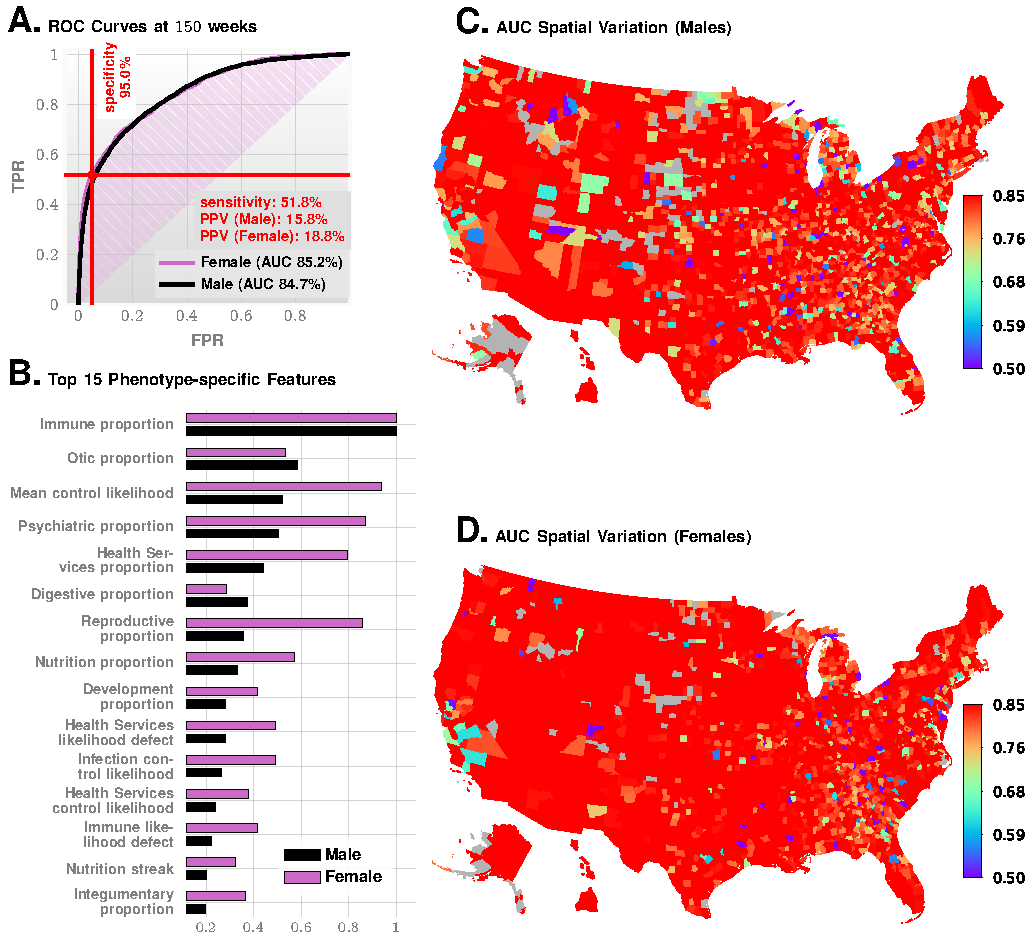
\includegraphics[width=0.99\textwidth]{Figures/External/main-figure0.pdf}
  \fi
     \vspace{-10pt}
 
     \captionN{ASD Occurrence Patterns. Panel A illustrates the spatial distribution of ASD insurance claims, and panel B shows the same data after population normalization, illustrating the relatively small demographic skew to ASD prevalence. %Panel C shows the recent dramatic increase in prevalence as reported by the CDC.
       Panel C illustrates the differential representation of different disease categories in the \treatment and control cohorts, and panel D shows the distribution of the age of  diagnosis for males and females. %Panel D illustrates the sparsity of the available codes for individual subjects.
     }\label{fig0}
\end{figure*}
\else
\refstepcounter{figure}\label{fig0}
\fi
%###########################################################
%###########################################################

%Our proposed approach is agnostic to parental educational level and language barriers, and is thus free from biases that have historically plagued questioinaire based screens~\cite{hyman2020identification}. Additionally, while M-CHAT/F is relatively easy and quick to administer, barriers to universal screening arising from the required  time and resource commitment from providers cannot be ignored~\cite{hyman2020identification}. These factors conspire  to produce reduced  coverage, which in turn has  cast  doubt upon the necessity and/or efficacy of universal screening programs~\cite{siu2016screening,pmid31562252} despite clear guidance on the contrary from the American Academy of Pediatricians (AAP)~\cite{hyman2020identification}. 

A  screening  tool that tracks the risk of an eventual ASD diagnosis,  based  on the information already being gathered during regular doctor's visits, and which may be implemented as a  fully automated background process requiring no time commitment from providers has the potential to reduce avoidable diagnostic  delays at no additional burden of time, money and personnel resources. 

While still lacking the certainty of a diagnostic blood test,  use of patterns emergent in  the diagnostic history to estimate risk might help reduce the subjective component in questionnaire-based screening tools, resulting in 1) reduced effect of potential language and cultural barriers in diverse populations, and 2) possibly better identify children with milder symptoms~\cite{hyman2020identification}.


Furthermore, being functionally independent of the M-CHAT/F, we show that there is clear advantage to combining the outcomes of the two tools: we can take advantage of any population stratification induced by the M-CHAT/F scores to significantly boost combined screening performance (See Methods, and Supplementary text, section~\ref{SI-sec:waittime}). 
%It may be more difficult to recognize mild symptoms of ASD in children younger than 3 years of age, especially if they have average or above-average cognitive abilities.  


%It is documented that observational tools are less effective in identifying  children with milder symptoms, use of patterns emergent in  the diagnostic history has the potential to be more effective in these borderline or uncertain scenarios.
%@@ RO1 --> Borderline scenarios

That such  predictions  of neuropsychiatric  disorders might be possible  from analyzing patterns in individual medical histories   is suggested by the fact  that  parents of children with ASD often notice a diagnosable developmental problem before their child's first birthday; while vision and hearing problems are not uncommon in the first year,  differences in social, communication, and fine motor skills have been reported to be  evident from about 6 months of age~\cite{pmid21410398,cdc}. The average population-level differences are immediately discernible $e.g.$, that  immunological disorders  and infections are much more common in children with autism, in any large database of patient diagnostic records (See Fig.~\ref{fig0}C).

Despite such reports,   a risk estimator that makes reliable predictions for  individuals | based purely on co-morbidity patterns |  has never been reported to the best of our knowledge. The sparsity of available diagnostic codes corresponding to 
individual subjects (See SI-Fig.~\ref{SI-figsparse}), and the general absence of physiological disorders  that would uniquely signal the eventual emergence of symptoms indicative of a clinical ASD diagnosis, combined with the heterogeneity of ASD presentation,  make such an endeavor challenging. In this study we report the  formulation of a principled  framework to make predictions 
based on models of statistically curated patterns of diagnostic code sequences automatically learned from  sufficiently large databases of electronic health records (EHR), that  achieves an out-of-sample AUC exceeding  $80\%$ for  either gender at  2.5 years (See Fig.~\ref{fig1}, and Fig.~\ref{fig2}A). 


We base our analysis on two independent  electronic databases of  diagnostic histories: the first one is a  claims database for private health insurance (Truven Marketscan), tracking over 5.6 million children between  2003 and 2012, and the second is the set of  de-identified diagnostic records  for nearly $70$ thousand children under 5 years of age treated at the  University of Chicago Medical Center between 2006 and 2018. The claims database is in good agreement with  documented prevalence: consistent with independent reports that ASD prevalence is  weakly dependent on demographic variables, and that  such effects are progressively diminishing~\cite{CDCdemo}, we find that  the distortion in the cartogram in  Fig.~\ref{fig0}A illustrating
 the spatial skew of  prevalence in our dataset largely disappears after population normalization (See Fig.~\ref{fig0}B). Additionally, in agreement with the widely studied  ASD comorbidity burden,  infections and immunological disorders have differential representation in the \treatment and control groups (See Fig.~\ref{fig0}C)
%, and  Table~\ref{tab0} in the main text  and SI-\ref{SI-tab0} in the Supplementary text for description of  the categories used in this study.) 
The  median diagnosis age is also comparable |  around 3 years in the claims database (See  Fig.~\ref{fig0}E)  versus 3 years 10 months for ASD in US~\cite{pmid29701730}. In this study, we refer to the cohort eventually diagnosed with autism as the ``positive'' cohort, as opposed to the control or the control cohort.

%Post-construction, we carry out extensive and rigorous cross-validation of our pipeline with held-back data. To test if our results are impacted by any unmodeled existing biases in the  Truven   database, we successfully re-validate our results with the de-identified medical records of approximately $70\times 10^3$ children treated at the University of Chicago Medical Center (UCM) between the years of 2006 and 2018.  

On the one hand, the use of machine learning limits us  to uncovering associations that may be learned statistically from data.
 On the other hand,  despite tremendous recent progress, efforts to  identify  causal biomarkers for ASD have had limited success. Currently,  over one hundred genes have been shown to contribute to autism risk~\cite{pmid26402605,pmid25038753,Satterstrom484113}, and it is  estimated that up to 1000 genes might be involved in ASD pathogenesis~\cite{pmid27891212}. Still, genetic interactions and mechanisms have accounted for a limited number of ASD cases~\cite{pmid18414403}, potentially implicating   environmental triggers that  work alongside genetic predispositions. The plausible sources of  risk are estimated to range from prenatal  factors such as maternal infection and inflammation, diet, and  household chemical exposures,  to autoimmune conditions and localized inflammation of the central nervous system after birth~\cite{pmid30971960,pmid30941018,pmid29691724,pmid29307081,pmid27351598,pmid26793298,pmid30095240,pmid25681541}. The heterogeneity of ASD presentation  admits the possibility of a plurality of   etiologies with converging pathophysiological pathways, making the investigation of the etiology of future risk modulation extremely challenging.

In our investigations  standard machine learning  tools failed to achieve clinically meaningful performance; the available data is too sparse for  off-the-shelf deep learning frameworks~\cite{pmid27185194} to make personalized predictions, and standalone classifiers or regressors fail to exploit the temporal dynamics embedded in the sparse diagnostic histories (See Section~\ref{SI-sec:offtheshelf} in the Supplementary text), requiring us to devise novel machine inference algorithms and feature engineering approaches to distill effective risk predictors (See Methods). 
%###########################################################
%###########################################################
%\ifFIGS
\begin{table}[t]
  \captionN{Disease Categories (A few ICD9 codes shown from the complete set of $9,835$ unique ICD9 codes considered. See SI-Table~\ref{SI-tab0} in  Supplementary text for complete list)}\label{tab0}
  \small\color{black!90}
  \begin{tabular}{L{1in}|L{2in} | |L{3in}}\hline
    \bf\sffamily   Category$^\dag$ & \bf\sffamily  Description  & \bf\sffamily  Examples of ICD9$^\star$ Codes \\\hline
\rowcolor{lightgray!80}ASD$^\star$ & Diagnostic Target & 299 299.0 299.00 299.01 299.9 299.8 299.91 299.90 299.80 299.81 299.1 299.10 299.11\\\hline
\cellcolor{Red1!70}Immunologic & Diseases related to dys-regulation of the Immune system &580.81 580.89 580.0 580.8 461 461.8 461.0 477.9 477.2 477 477.8\\\hline
\cellcolor{Red1!70}Infectious & Diseases Caused By Pathogens &487.8 488.12 488.0 488.01 487.0 487.1 488.09 464.4 466 466.11 466.1\\\hline
 \cellcolor{Red1!50}Nutrition &  Symptoms concerning nutrition, metabolism and development   & 783.0 783.21 783.3 783.40 783.42 783.7 783.9\\\hline
   \cellcolor{Red1!50}Mental Disorders & Psychiatric phenotypes other than ASD & 290 -  319 (except 299.x) \\\hline
    \cellcolor{Red1!50}Health Services &Contact With   Health Services and Classification Of Factors Influencing Health Status  & V01.0 V01.1 V01.2 V01.3 V01.4   V09.70 V09.71 V88.02 V88.03 V89.01 V89.02 V89.03 V89.04 V89.05 V89.09 \\\hline
    \cellcolor{IndianRed1!50}Digestive & Diseases Of The Digestive System &540.0 540.1 541.0 542 540 541 543.0 562.03 562.01 562.00 562.10\\\hline
\cellcolor{IndianRed1!50}Otic & Diseases Of The Ear And Mastoid Process
 &381.51 381.50 381.81 381.89 381.61 381.62 381 381.7 385.82 383.32 380.30\\\hline
\cellcolor{IndianRed1!50}Musculoskeletal & Congenital musculoskeletal anomalies &756.52 756.53 733.02 733.0 733.09 737.43 737.41 737.20 737.29 737.4 737.2\\\hline
    \cellcolor{IndianRed1!50}Developmental & Congenital  anomalies (Non-overlapping with muskuloskeletal)  &755.55 743.45 743.11 743.10 743.00 743.03 743.44 743.22 743.20 743.21 758.4\\\hline
    \cellcolor{IndianRed1!30}Reproductive & Diseases Of The Genitourinary System   &611.79 611.71 611.89 611.81 676.64 611 676.60 611.6 611.4 611.3 611.2\\\hline
    \cellcolor{IndianRed1!20}Integumentary & Diseases Of Skin And Subcutaneous Tissue &706.0 706.1 704.00 704.02 704.09 680.9 680.1 680.5 680.7 680.6 680\\\hline
    %
    Ophthalmologic & Disorders Of The Eye And Adnexa &362.8 362.9 362.6 362.1 362.3 362.18 362.17 362.13 362.11 363.33 363.32\\\hline
 Hematologic &  Diseases Of The Blood And Blood-Forming Organs & 286.9 286.6 283.19 283.11 283.9 283.1 284.0 284.09 284 284.01\\\hline
Metabolic & Metabolic Disorders (Non-overlapping with respiratory, digestive and immunological conditions) &273.4 270 270.3 712.11 712.13 712.12 712.14 712.18 712.30 712.37 712.36\\\hline
Cardiovascular & Diseases Of Arteries, Arterioles, And Capillaries  &442.89 441.6 442.82 442.83 441.03 441.02 441.00 442 414.11 447.70 447.71\\\hline
    Respiratory & Diseases Of The Respiratory System (non-overlapping with Infectious) &516.31 516.30 516.32 516.35 516.37 516.36 516.8 516.0 277.0 277.00 277.01\\\hline
Endocrine & Disorders Of Thyroid and other Endocrine Glands &244 244.9 244.2 255.41 255.5 255.4 259.51 255 259.4 255.11 242.2\\\hline
  \end{tabular}
  \vskip 1em
  \small
  $^\dag$ Categories inferred to be   important for risk modulation are proportionately highlighted.\\
  $^\star$ ICD10 codes when present were mapped back to closest ICD9 matches using published General Equivalence Mappings~\cite{GEMS}.
\end{table}
% \else
% \refstepcounter{table}\label{tab0}
% \fi
%###########################################################
%###########################################################
%###########################################################


%###########################################################
%\ifFIGS
\begin{table}[t]
  \captionN{Engineered Features (Total Count: 165)}\label{tab1}
\begin{tabular}{L{2.25in}|L{3in}|C{1in}} \hline
\textbf{Feature Type$^\ddag$}               & \textbf{Description}   & \textbf{No. of Features}   \\\hline
{[}Disease Category{]}$_{ \ \Delta}$               & Likelihood Defect (See Methods section) & 17   \\\hline
  {[}Disease Category{]}$_{ \ 0}$               & Likelihood of control model (See Methods section) & 17  \\\hline
{[}Disease Category{]}$_{\textrm{ proportion}}$   & Occurrences in the encoded sequence / length of the sequence         & 17\\\hline
{[}Disease Category{]}$_{\textrm{ streak}}$      & Maximum Length of adjacent occurrences  of {[}Disease Category{]}    & 51      \\\hline
{[}Disease Category{]}$_\textrm{ prevalence}$   &  Maximum, mean  and variance of Occurrences in the encoded sequence / Total Number of diagnostic codes in the mapped sequence   & 51      \\\hline
  Feature Mean, Feature Variance, Feature Maximum for difference of control and case models                 & Mean, Variance, Maximum of the {[}Disease Category{]}$_{ \ \Delta}$ values   & 3     \\\hline
  Feature Mean, Feature Variance, Feature Maximum for control models               & Mean, Variance, Maximum of the {[}Disease Category{]}$_{\ 0}$ values   & 3     \\\hline
Streak      & Maximum, mean  and variance of the length of adjacent occurrences  of {[}Disease Category{]}    & 3      \\\hline
Intermission& Maximum, mean  and variance of the length of adjacent empty weeks     & 3    \\\hline
\end{tabular}
\vskip 1em
\small
$^\ddag$ Disease categories are described in Table~\ref{tab0}
\end{table}
% \else
% \refstepcounter{table}\label{tab1}
% \fi
%###########################################################
%###########################################################
%###########################################################
\section*{Materials \& Methods}
%##########################################
%##########################################
%###########################################################
% ###########################################################
\ifFIGS
\begin{figure*}[!t]
  \tikzexternalenable
  \centering  
  \vspace{-10pt}
  
\def\DATA{../data_revision}
\iftikzX
  \input{Figures/figpred1_}
  \else
  \includegraphics[width=0.99\textwidth]{Figures/External/main-figure1.pdf}
  \fi
     \vspace{-5pt}

     \captionN{Predictive Performance. Panels A and B show the spatial variation in the achieved predictive performance at 150 weeks, measured by AUC, for males and females, respectively. Gray areas lack data on either positive or negative cases. Panel %C shows the distribution of the AUC, and panel
       C shows the ROC curves for males and females. Panel D shows the feature importance inferred by our prediction pipeline. The detailed description of the features is given in Table~\ref{tab0}. The most import feature is related to immunologic disorders, and we note that in addition to features related to individual disease categories, we also have the mean control likelihood (rank 3), which may be interpreted as the average likelihood of the diagnostic patterns correspond to the control category as opposed to the \treatment category.
       % The most important feature for prediction is \textit{feature mean} and \textit{feature variance}, which are the mean and variance of our novel stochastic automata based metric, averaged over 18 phenotypically and etiologically distinct disease categories.
     }\label{fig1}
\end{figure*}
\else
\refstepcounter{figure}\label{fig1}
\fi
%###########################################################
%###########################################################
%###########################################################
%###########################################################
%###########################################################
\ifFIGS
\begin{figure*}[!ht]
  \tikzexternalenable
  \vspace{-15pt}
  
  \centering 
 \def\DATA{../data_revision}
\iftikzX
  \input{Figures/figpred2_}
  \else
   \includegraphics[width=0.99\textwidth]{Figures/External/main-figure2.pdf}
   \fi
   \vspace{-10pt}

    \captionN{More details on Predictive Performance and Variation of Inferred Risk. Panel A illustrates AUC achieved as a function of
      patient age, for the Truven and UCM datasets. The shaded area outlines the 2 - 2.5  years of age, and  shows that we achieve $>80\%$ AUC for either gender from shortly afer 2 years. Panel B illustrates  how inferred models differ between the control vs. the \treatment cohorts. On average, models get less complex, implying the exposures get more statistically independent.  Panel C illustrates how the average risk changes with time for the control and the positive cohorts. Panel D shows the distribution of the prediction horizon: the time to a clinical diagnosis after inferred  relative risk crosses $90\%$. Panel E shows that for each new disease code for a low-risk child, ASD risk increases by approximately $2\%$ for either gender. Panel F illustrates the risk progression of a specific, ultimately autistic male child in the Truven database. Abbreviations in the legend: ill defn. (Symptoms, Signs, And Ill-Defined Conditions),   musc. skltl. (Diseases Of The Musculoskeletal System And Connective Tissue), cond. orig. in perintl. (Certain Conditions Originating In The Perinatal Period), immun. (Endocrine, Nutritional And Metabolic Diseases, And Immunity Disorders), nerv. \& sensory (Diseases Of The Nervous System And Sense Organs), respir. (Respiratory Disorders), and digest. (Digestive Disorders).}\label{fig2}
\end{figure*}
\else
\refstepcounter{figure}\label{fig2}
\fi
%###########################################################
%###########################################################

%###########################################################
\ifFIGS
%###########################################################
\begin{figure*}[!ht]
  \tikzexternalenable
  \vspace{-10pt}
  
\pgfplotsset{
  discard if/.style 2 args={
    x filter/.append code={
      \edef\tempa{\thisrow{#1}}
      \edef\tempb{#2}
      \ifx\tempa\tempb
      \def\pgfmathresult{inf}
      \fi
    }
  },
  discard if not/.style 2 args={
    x filter/.append code={
      \edef\tempa{\thisrow{#1}}
      \edef\tempb{#2}
      \ifx\tempa\tempb
      \else
      \def\pgfmathresult{inf}
      \fi
    }
  }
}

\begin{tikzpicture}[font=\bf\sffamily\fontsize{8}{10}\selectfont]
  \def\TEXTCOL{gray}

%\draw[fill=gray,opacity=.1]
\clip (-4.65in,-2.35in) rectangle (2.2in,3in);
  
\def\DATAPATH{../../revision_results/roc/restricted_neg_len/RAW/}
\def\datafile{\DATAPATH/CHOP_PRC_pipeline_BASIC_M_100w.csv}
\def\datafilef{\DATAPATH/CHOP_PRC_pipeline_BASIC_F_100w.csv}
\def\vdatafile{\DATAPATH/CHOP_PRC_valid_BASIC_M_100w.csv}  
\def\vdatafilef{\DATAPATH/CHOP_PRC_valid_BASIC_F_100w.csv}
  \def\datafileQ{\DATAPATH/thisRFall.csv}

  \def\AXISCOL{white}
  \def\BANDCOL{lightgray}
  \def\PLOTCOLA{black}
  \def\PLOTCOLB{\MXCOL}
  \def\PLOTCOLBu{\MXCOL}
  \def\PLOTCOLC{black}
  \def\PLOTCOLD{\FXCOL}
  \def\FNCOLB{SeaGreen2}
  \def\PLOTCOLDu{\FXCOL}
  \def\WDTa{1.65in}
  \def\HGTa{1.45in}

  \def\SCALE{1.5}
  \def\SCALEA{1.25}
  \def\SCALEB{.9}
  \def\OPC{.75}
  \def\OPCB{.95}
  \def\BWIDTH{4pt}
  \def\LWDT{0.5mm}

  \def\LWDT{0.8mm}
  \def\SKIP{4}
  \def\HGT{1.625in}
  \def\WDT{1.8in}

  \tikzstyle{mopt} = [ scale=\SCALEB, , opacity=0,fill opacity=1,] 
  % \pgfplotsset{
  %   % colormap/hot,
  % colormap/viridis,
  % % colormap={reverse winter}{
  % % indices of colormap={
  % % \pgfplotscolormaplastindexof{YlGnBu},...,0 of YlGnBu}
  % % },
  % }
  \pgfplotsset{
    colormap={hot}{color(0cm)=(Orchid1); 
      color(1cm)=(DodgerBlue1); 
      color(2cm)=(DodgerBlue2); 
      color(3cm)=(orange); 
      color(4cm)=(DarkOrange1); 
      color(5cm)=(Yellow2)}
  }
  \pgfplotsset{
    colormap={hot}{color(0cm)=(MidnightBlue); 
      color(1cm)=(CadetBlue2!90!black); 
      color(2cm)=(CadetBlue1!93!black); 
      color(3cm)=(Bisque1!93!black); 
      color(4cm)=(DarkOrange1); 
      color(5cm)=(Yellow2!98!black)}
  }
  \node[] (A) {
    \begin{tikzpicture}[anchor=center,
      font=\bf\sffamily\fontsize{8}{10}\selectfont]
      \begin{groupplot}[name=Agg,
        group style={
          group name=Ag,
          group size=2 by 2,
          xlabels at=edge bottom,
          xticklabels at=edge bottom,
          vertical sep=.55in,
          horizontal sep=.55in,
        },% colormap={reverse winter}{
        % indices of colormap={
        % \pgfplotscolormaplastindexof{Spectral},...,0 of Spectral}
        % },
        grid style={thick,dashed, gray!40},%,point meta min=.9,point meta max=1,colorbar,
        % ymax=0.855
        ,legend cell align={left},
        legend style={anchor=east,at={(0.25,1.1)},
          inner sep=3pt,
          draw=none,
          fill=white,fill opacity=.850,
          align=left,anchor=west,
          text opacity=1,
          font=\bf\sffamily\fontsize{8}{9}\selectfont,text=black},
        grid style={thick,dashed, gray!40},
        grid,
        enlargelimits=false,scale only axis=true,
        scaled x ticks = false,scaled y ticks = false,
        axis line style={\AXISCOL, opacity=1,ultra  thick, 
          rounded corners=0pt}, 
        y tick label style={/pgf/number format/fixed,
          /pgf/number format/precision=2,/pgf/number format/fixed zerofill,
          /pgf/number format/1000 sep = %\thinspace % Optional to replace comma as the 1000 separator 
        },
        major tick length=0pt,legend columns=1, 
        legend style={,xshift=-.5in,yshift=.2in},
        xlabel={},xticklabel style={yshift=-.05in},
        xlabel style={yshift=0.1in},ylabel
        style={xshift=-1in},ylabel={PPV},
        grid style={thick,dashed, gray!40},
        point meta min=0.92, point meta max=0.98,
        title style={yshift=.0in,xshift=-.2in,align=left}]

        \nextgroupplot[ymin=0.14,ymax=.35,xmin=.35,xmax=.65,text=\TEXTCOL, height=\HGTa,
        width=\WDTa,title={{\Large i.} 24 month, Male Truven}]
        \addplot[only marks,scatter,scatter src=explicit, mark options={%
          mopt,
        },]table[col sep=comma,x=s, y=p,meta=c]
        {\datafile};
        \node[,thick,anchor=center,] (x1t) at (axis cs:.388,0.145) {};
        \node[thick,anchor=center,] (x2t) at (axis cs:.388,0.29) {};
        \node[thick,anchor=center,] (x3t) at (axis cs:.54,0.162) {};

        \nextgroupplot[ymin=0.14,ymax=.35,xmin=.35,xmax=.65,text=\TEXTCOL, height=\HGTa,
        width=\WDTa,ylabel={},title={{\Large ii.} 24 month, Female Truven}]
        \addplot[only marks,scatter,scatter src=explicit, mark options={%
          mopt,
        },]table[col sep=comma,x=s, y=p,meta=c]
        {\datafilef};
        \node[,thick,anchor=center,] (x1) at (axis cs:.388,0.145) {};
        \node[thick,anchor=center,] (x2) at (axis cs:.388,0.35) {};
        \node[thick,anchor=center,] (x3) at (axis cs:.57,0.17) {};
        % \draw[->,>=stealth',thick,dashed] (x1) -- (x2);
        % \addplot[mark=*, only marks, mark options={scale=.4,fill=black}]table[col sep=comma,x=s, y=p]
        % {\datafileHp};

        \nextgroupplot[ymin=0.14,ymax=.35,xmin=.35,xmax=.65,text=\TEXTCOL, height=\HGTa,
        width=\WDTa,ylabel={}, ,title={{\Large iii.} 24 month, Male UCM}]
        \addplot[only marks,scatter,scatter src=explicit, mark options={%
          mopt,
        },]table[col sep=comma,x=s, y=p,meta=c]
        {\vdatafile};
        \node[,thick,anchor=center,] (x1u) at (axis cs:.388,0.145) {};
        \node[thick,anchor=center,] (x2u) at (axis cs:.388,0.35) {};
        \node[thick,anchor=center,] (x3u) at (axis cs:.63,0.15) {};

        \nextgroupplot[ymin=0.14,ymax=.35,xmin=.35,xmax=.65,text=\TEXTCOL, height=\HGTa,
        width=\WDTa,ylabel={}, extra x ticks={.3},,title={{\Large iv.} 24 month, Female UCM}]
        \addplot[only marks,scatter,scatter src=explicit, mark options={%
          mopt,
        },]table[col sep=comma,x=s, y=p,meta=c]
        {\vdatafilef};
        \node[,thick,anchor=center,] (x1f) at (axis cs:.388,0.145) {};
        \node[thick,anchor=center,] (x2f) at (axis cs:.388,0.31) {};
        \node[thick,anchor=center,] (x3f) at (axis cs:.62,0.15) {};
      \end{groupplot}

      \node[draw=IndianRed1,fill=none,thick,anchor=center,
      label={[text=IndianRed1]0:HP$^\dag$}] (x2t) at (x2t) {}; 
      \node[draw=IndianRed1,fill=none,thick,anchor=center,
      label={[text=IndianRed1,fill=white]80:HR$^\dag$}] (x3t) at (x3t) {};
      \draw[-{latex},IndianRed1,ultra thick,dashed] (x1t) -- (x2t);
      \draw[-{Latex},IndianRed1,ultra thick,dashed] (x1t) -- (x3t);
      \node[draw=IndianRed4,fill=IndianRed2,thick,anchor=center,
      label={[text=IndianRed1,fill=white,font=\bf\sffamily\fontsize{6}{7}\selectfont,
        label distance=0.02in]-120:MCHAT-F}] (x1t) at (x1t) {};


      \node[draw=IndianRed1,fill=none,thick,anchor=center,label={[text=IndianRed1]0:HP$^\dag$}] (x2u) at (x2u) {}; 
      \node[draw=IndianRed1,fill=none,thick,anchor=center,
      label={[text=IndianRed1,fill=white]80:HR$^\dag$}] (x3u) at (x3u) {};
      \draw[-{latex},IndianRed1,ultra thick,dashed] (x1u) -- (x2u);
      \draw[-{Latex},IndianRed1,ultra thick,dashed] (x1u) -- (x3u);
      \node[draw=IndianRed4,fill=IndianRed2,thick,anchor=center,label={[text=IndianRed1,
        fill=white,font=\bf\sffamily\fontsize{6}{7}\selectfont,
        label distance=0.02in]-120:MCHAT-F}] (x1u) at (x1u) {};



      \node[draw=IndianRed1,fill=none,thick,anchor=center,
      label={[text=IndianRed1]0:HP$^\dag$}] (x2) at (x2) {}; 
      \node[draw=IndianRed1,fill=none,thick,anchor=center,
      label={[text=IndianRed1,fill=white]80:HR$^\dag$}] (x3) at (x3) {};
      \draw[-{latex},IndianRed1,ultra thick,dashed] (x1) -- (x2);
      \draw[-{Latex},IndianRed1,ultra thick,dashed] (x1) -- (x3);
      \node[draw=IndianRed4,fill=IndianRed2,thick,anchor=center,
      label={[text=IndianRed1,fill=white,font=\bf\sffamily\fontsize{6}{7}\selectfont,
        label distance=0.02in]-120:MCHAT-F}] (x1) at (x1) {};


      \node[draw=IndianRed1,fill=none,thick,anchor=center,
      label={[text=IndianRed1]0:HP$^\dag$}] (x2f) at (x2f) {};
      \node[draw=IndianRed1,fill=none,thick,anchor=center,
      label={[text=IndianRed1,fill=white]90:HR$^\dag$}] (x3f) at (x3f) {};
      \draw[-{latex},IndianRed1,ultra thick,dashed,opacity=1] (x1f) -- (x2f);
      \draw[-{Latex},IndianRed1,ultra thick,dashed,opacity=1] (x1f) -- (x3f);
      \node[draw=IndianRed4,fill=IndianRed2,thick,anchor=center,
      label={[text=IndianRed1,fill=white,font=\bf\sffamily\fontsize{6}{7}\selectfont,
        label distance=0.02in]-120:MCHAT-F}] (x1f) at (x1f) {};
    \end{tikzpicture}};

  \node[anchor=north east] (B) at ([yshift=.65in,xshift=-.1in]A.north west)
  {
  \def\TEXTCOL{gray}

  \def\DATAPATH{../../revision_results/roc/restricted_neg_len/RAW/}
  \def\datafile{\DATAPATH/RAWPRCpipeline_BASIC_M_150w.csv}
  \def\datafileF{\DATAPATH/RAWPRCpipeline_BASIC_F_150w.csv}
  \def\datafileU{\DATAPATH/RAWPRCvalid_BASIC_M_150w.csv}
  \def\datafileUF{\DATAPATH/RAWPRCvalid_BASIC_F_150w.csv}

  \def\datafileh{\DATAPATH/RAWPRCpipeline_BASIC_M_100w.csv}
  \def\datafileFh{\DATAPATH/RAWPRCpipeline_BASIC_F_100w.csv}
  \def\datafileUh{\DATAPATH/RAWPRCvalid_BASIC_M_100w.csv}
  \def\datafileUFh{\DATAPATH/RAWPRCvalid_BASIC_F_100w.csv}

  \def\AXISCOL{white}
  \def\HGT{1.55in}
  \def\WDT{1.6in}
  \def\MXCOLB{gray}
  \def\FXCOLB{CadetBlue3}
  \def\OPC{.75}
  \def\OPCB{.65}
  \def\LWDT{.8mm}
  \def\SKIP{7}

    \begin{tikzpicture}[text=\TEXTCOL, ]
      \begin{groupplot}
        [name=Agg,
        group style={
          group name=Ag,
          group size=1 by 2,
          %xlabels at=edge bottom,
          %xticklabels at=edge bottom,
          vertical sep=.8in,
          % horizontal sep=.55in,
        },        ,legend cell align={left},
        legend style={anchor=east,at={(-0.25,1.1)},
          inner sep=3pt,
          draw=none,
          fill=white,fill opacity=.850,
          align=left,anchor=west,
          text opacity=1,
          font=\bf\sffamily\fontsize{8}{9}\selectfont,text=black},legend columns=2, 
        name=K,
        clip=true,,
        width=\WDT,
        height=\HGT,
        scale only axis=true,
        enlargelimits=false,
        axis on top=false,
        % axis background/.style={
        %   shade,top color=transparent!5,bottom color=transparent!5},
        axis line style={\AXISCOL, opacity=1,ultra  thick, 
          rounded corners=0pt}, 
        grid,
        grid style={thick,dashed, gray!40},
         xticklabel style={yshift=-.05in},
        xlabel style={yshift=-.075in,text=\TEXTCOL},
        ylabel style={align=center,,text=\TEXTCOL,anchor=center,
          yshift=-.175in},
        % tickpos=left,
        ytick align=outside,
        xtick align=outside,
        major tick length=0pt,
        scaled y ticks = false,
        y tick label style={/pgf/number format/fixed,
          /pgf/number format/1000 sep = \thinspace % Optional if you00 separator 
        },
        ylabel={PPV},xlabel={sensitivity (TPR)},title style={text=\TEXTCOL, yshift=.25in,xshift=-1.25in,anchor=south west},
        % extra x ticks={1},extra x tick labels={1}
        ]

        \nextgroupplot[ xlabel={}, xmin=0.03, ymax=0.7,title={{\Large i. } 150 weeks},]
        \addplot [each nth point=\SKIP, filter discard warning=false, 
        unbounded coords=discard,smooth,draw=\MXCOL, line width=\LWDT,opacity=\OPC,
        ]table [col sep=comma,x=tpr,y=p] {\datafile};
        \addlegendentry{Male Truven}

        \addplot [each nth point=\SKIP, filter discard warning=false, 
        unbounded coords=discard,smooth,draw=\FXCOL,  line width=\LWDT,,opacity=\OPC,
        ]table [col sep=comma,x=tpr,y=p] {\datafileF};
        \addlegendentry{Female Truven}

        \addplot [each nth point=\SKIP, filter discard warning=false, 
        unbounded coords=discard,smooth,draw=\MXCOLB,  line width=\LWDT,,opacity=\OPC,
        ]table [col sep=comma,x=tpr,y=p] {\datafileU};
        \addlegendentry{Male UCM}

        \addplot [each nth point=\SKIP, filter discard warning=false, 
        unbounded coords=discard,smooth,draw=\FXCOLB,  line width=\LWDT,,opacity=\OPC,
        ]table [col sep=comma,x=tpr,y=p] {\datafileUF};
        \addlegendentry{Female UCM}


        \nextgroupplot[ xlabel={sensitivity (TPR)},xmin=0.03, ymax=0.7,,title={{\Large ii. } 100 weeks}]
        \addplot [each nth point=\SKIP, filter discard warning=false, 
        unbounded coords=discard,smooth,draw=\MXCOL, line width=\LWDT,,opacity=\OPC,
        ]table [col sep=comma,x=tpr,y=p] {\datafileh};
        \addlegendentry{Male Truven}

        \addplot [each nth point=\SKIP, filter discard warning=false, 
        unbounded coords=discard,smooth,draw=\FXCOL,  line width=\LWDT,,opacity=\OPC,
        ]table [col sep=comma,x=tpr,y=p] {\datafileFh};
        \addlegendentry{Female Truven}

        \addplot [each nth point=\SKIP, filter discard warning=false, 
        unbounded coords=discard,smooth,draw=\MXCOLB,  line width=\LWDT,,opacity=\OPC,
        ]table [col sep=comma,x=tpr,y=p] {\datafileUh};
        \addlegendentry{Male UCM}

        \addplot [each nth point=\SKIP, filter discard warning=false, 
        unbounded coords=discard,smooth,draw=\FXCOLB,  line width=\LWDT,,opacity=\OPC,
        ]table [col sep=comma,x=tpr,y=p] {\datafileUFh};
        \addlegendentry{Female UCM}
      \end{groupplot}\end{tikzpicture}
  };
% \node[anchor=north] (CC) at ($(A.south east)!.5!(B.south west)$) {\begin{tikzpicture}[font=\bf\sffamily\fontsize{8}{10}\selectfont]
%   \def\TEXTCOL{gray}
%   \def\DATAPATH{../../revision_results/roc/restricted_neg_len/RAW/}
%   \def\datafile{\DATAPATH/thisRFall.csv}
%   \def\AXISCOL{white}
%   \def\WDTa{1.85in}
%   \def\HGTa{2in}
%   \def\HGT{1.2in}
%   \def\WDT{1.2in}
%   \def\MXCOLB{gray}
%   \def\FXCOLB{CadetBlue3}
%   \def\OPC{.75}
%   \def\OPCB{.65}
%   \def\LWDT{0.8mm}
%   \def\SKIP{4}
%   \node[] (A0) at (0,0) {};
%   \node[anchor=center] (N) at (A0.south)
%   {
%     \begin{tikzpicture}[text=\TEXTCOL, ]
%       \begin{groupplot}
%         [name=Agg,
%         group style={
%           group name=Ag,
%           group size=3 by 1,
%           xlabels at=edge bottom,
%           xticklabels at=edge bottom,
%           vertical sep=.75in,
%           horizontal sep=.9in,
%         },        ,legend cell align={left},
%         legend style={anchor=east,at={(-0.12,1.1)},
%           inner sep=3pt,
%           draw=none,
%           fill=white,fill opacity=.850,
%           align=left,anchor=west,
%           text opacity=1,
%           font=\bf\sffamily\fontsize{8}{9}\selectfont,text=black},legend columns=2, 
%         name=K,
%         clip=true,,
%         width=\WDT,
%         height=\HGT,
%         scale only axis=true,
%         enlargelimits=false,
%         axis on top=false,
%         % axis background/.style={
%         % shade,top color=transparent!5,bottom color=transparent!5},
%         axis line style={\AXISCOL, opacity=1,ultra  thick, 
%           rounded corners=0pt}, 
%         grid,
%         grid style={thick,dashed, gray!40},
%         % xticklabel style={xshift=0.05in,yshift=-.05in},
%         xlabel style={yshift=.05in,text=\TEXTCOL},
%         ylabel style={align=center,,text=\TEXTCOL,anchor=center,
%           yshift=-.175in},
%         % tickpos=left,
%         ytick align=outside,
%         xtick align=outside,
%         major tick length=0pt,
%         scaled y ticks = false,
%         y tick label style={/pgf/number format/fixed,
%           /pgf/number format/1000 sep = \thinspace % Optional if you00 separator 
%         },
%         ylabel={PPV},xlabel={sensitivity (TPR)},point meta=explicit,
%         colorbar style={width=.1in,y tick label style={/pgf/number format/fixed,/pgf/number format/precision=3,/pgf/number format/fixed zerofill,
%             /pgf/number format/1000 sep = %\thinspace % Optional if you want to replace comma as the 1000 separator 
%           },}
%         ]

%         \nextgroupplot[colorbar]
%         \pgfplotsset{
%           colormap={hot}{color(0cm)=(MidnightBlue); color(1cm)=(CadetBlue2!90!black); color(2cm)=(CadetBlue1!93!black); color(3cm)=(Bisque1!93!black); color(4cm)=(DarkOrange1); color(5cm)=(Yellow2!93!black)}
%         }
%         \addplot [mesh, very thick, %point meta min=0.92, point meta max=0.98
% ]table [col sep=comma,x=s,y=p,meta=c,
%         % discard if not={gender}{M},
%         restrict expr to domain={\thisrow{c}}{0.966:1},restrict expr to domain={\thisrow{rho}}{0.012:1}] {\datafile};

%         \nextgroupplot[colorbar,ylabel={}]
%         \pgfplotsset{
%           colormap={hot}{color(0cm)=(lightgray!70); color(1cm)=(lightgray!80); color(2cm)=(lightgray!80!Bisque1); color(3cm)=(Bisque1!90!Tomato); color(4cm)=(Tomato); color(5cm)=(Red1)}
%         }
%         \addplot [mesh, very thick]table [col sep=comma,x=s,y=p,meta=rho,
%         % discard if not={gender}{M},
%         restrict expr to domain={\thisrow{c}}{0.966:1},restrict expr to domain={\thisrow{rho}}{0.012:1}] {\datafile};

%         \nextgroupplot[colorbar,ylabel={}]
%         \pgfplotsset{
%           colormap={hot}{color(0cm)=(lightgray!70); color(1cm)=(lightgray!80); color(2cm)=(lightgray!80!Bisque1); color(3cm)=(Bisque1!90!Tomato); color(4cm)=(Tomato); color(5cm)=(Red1)}
%         }
%         \addplot [mesh, very thick]table [col sep=comma,x=rs,y=tm,meta=rho,
%         discard if not={gender}{M},
%         restrict expr to domain={\thisrow{c}}{0.95:1},
%         restrict expr to domain={\thisrow{rho}}{0.016:0.0224},
%         restrict expr to domain={\thisrow{rs}}{1:1.5},
%         ] {\datafile};
%       \end{groupplot}
%     \end{tikzpicture}
%   };
%\end{tikzpicture}
%};
 

  \node[anchor=north,font=\bf\sffamily\fontsize{8}{10}\selectfont,
  text=\TEXTCOL] (CC) at ([yshift=0in]A.south) {sensitivity (TPR)};

  \node[anchor=south] (CB) at ([yshift=.05in]A.north) {
    \begin{tikzpicture}[font=\bf\sffamily\fontsize{8}{10}\selectfont,
      text=\TEXTCOL]
      \begin{axis}[,
        hide axis,
        scale only axis,
        height=0pt,
        width=0pt,
        colorbar horizontal,
        point meta min=0.92,
        point meta max=0.98,
        colorbar style={
          title={specificity},title style={yshift=-.1in},
          width=3in,
          height=.15in,
          xticklabel style={yshift=-.05in},
          xtick={0.92,0.93,0.94,.95,0.96,0.97,0.98}
        }]
        \addplot [draw=none] coordinates {(0,0)};
      \end{axis}
    \end{tikzpicture}};

  \node[anchor=south west] (L1) at ([xshift=-.05in]CB.north west) {{\Large B.} 4D  Optimization Conditioned  on MCHAT-F To Boost Performance$^\ddag$};
 \node[anchor=south west] (L2) at ([xshift=.75in,yshift=-.01in]$(L1.south west) !(B.west)!(L1.south east)$) {{\Large A.} PPV/Sesnitivity or Precision/Recall Curves};

\end{tikzpicture}

 
 \vspace{0pt}
  
\pgfplotsset{
    discard if/.style 2 args={
        x filter/.append code={
            \edef\tempa{\thisrow{#1}}
            \edef\tempb{#2}
            \ifx\tempa\tempb
                \def\pgfmathresult{inf}
            \fi
        }
    },
    discard if not/.style 2 args={
        x filter/.append code={
            \edef\tempa{\thisrow{#1}}
            \edef\tempb{#2}
            \ifx\tempa\tempb
            \else
                \def\pgfmathresult{inf}
            \fi
        }
    }
  }

  \begin{tikzpicture}[font=\bf\sffamily\fontsize{8}{10}\selectfont]
  \def\TEXTCOL{gray}

  \def\DATAPATH{../../revision_results/roc/restricted_neg_len/RAW/}
  \def\datafile{\DATAPATH/thisRFall.csv}


  \def\AXISCOL{white}
  \def\WDTa{1.85in}
  \def\HGTa{2in}
  \def\HGT{1.2in}
  \def\WDT{1.2in}
  \def\MXCOLB{gray}
  \def\FXCOLB{CadetBlue3}
  \def\OPC{.75}
  \def\OPCB{.65}
  \def\LWDT{0.7mm}
  \def\SKIP{4}  
  \def\WDTa{1.75in}
  \def\WDTb{1.25in}
  \def\HGTa{1.65in}
  \def\SKIP{5}
  \def\SKIPB{1}
  \def\LCOL{black}

  \node[] (A0) at (0,0) {};
  \node[anchor=center] (N) at (A0.south)
  {
    \begin{tikzpicture}[text=\TEXTCOL, ]
      \begin{groupplot}
        [name=Agg,
        group style={
          group name=Ag,
          group size=3 by 1,
          xlabels at=edge bottom,
          xticklabels at=edge bottom,
          vertical sep=.75in,
          horizontal sep=.8in,
        },        ,legend cell align={left},
        legend style={anchor=east,at={(-0.12,1.1)},
          inner sep=3pt,
          draw=none,
          fill=white,fill opacity=.850,
          align=left,anchor=west,
          text opacity=1,
          font=\bf\sffamily\fontsize{8}{9}\selectfont,text=black},legend columns=2, 
        name=K,
        clip=true,,
        width=\WDTa,
        height=\HGTa,
        scale only axis=true,
        enlargelimits=false,
        axis on top=false,
        % axis background/.style={
        %   shade,top color=transparent!5,bottom color=transparent!5},
        axis line style={\AXISCOL, opacity=1,ultra  thick, 
          rounded corners=0pt}, 
        grid,
        grid style={thick,dashed, gray!40},
        % xticklabel style={xshift=0.05in,yshift=-.05in},
        xlabel style={yshift=.05in,text=\TEXTCOL},
        ylabel style={align=center,,text=\TEXTCOL,anchor=center,
          yshift=-.15in},
        % tickpos=left,
        ytick align=outside,
        xtick align=outside,
        major tick length=0pt,
        scaled y ticks = false,
        y tick label style={/pgf/number format/fixed,
          /pgf/number format/1000 sep = \thinspace % Optional if you00 separator 
        },
        ylabel={PPV},xlabel={sensitivity (TPR)},point meta=explicit,
        colorbar style={width=.1in,y tick label style={/pgf/number format/fixed,/pgf/number format/precision=2,/pgf/number format/fixed zerofill,
     /pgf/number format/1000 sep = %\thinspace % Optional if you want to replace comma as the 1000 separator 
      },}
        % extra x ticks={1},extra x tick labels={1}
        ]

   \nextgroupplot[colorbar horizontal,xmin=.98,extra x ticks={1},colorbar style={at={(0,1.2)},title={prevalence},title style={yshift=-.1in},
          height=.1in,scaled x ticks=false,
x tick label style={/pgf/number format/fixed,
          /pgf/number format/precision=3,/pgf/number format/fixed zerofill,
          /pgf/number format/1000 sep = %\thinspace % Optional to replace comma as the 1000 separator 
        },
          xticklabel style={yshift=-.025in},},ylabel={MCHAT-F relative wait time},xlabel={MCHAT-F relative sensitivity}]
        \pgfplotsset{
colormap={hot}{color(0cm)=(lightgray!70); color(1cm)=(lightgray!80); color(2cm)=(lightgray!80!Bisque1); color(3cm)=(Bisque1!90!Tomato); color(4cm)=(Tomato); color(5cm)=(Red1)}
}
\addplot [mesh, each nth point=\SKIP, filter discard warning=false, 
        unbounded coords=discard,line width=\LWDT]table [col sep=comma,x=rs,y=tm,meta=rho,
discard if not={gender}{M},
restrict expr to domain={\thisrow{c}}{0.95:1},
restrict expr to domain={\thisrow{rho}}{0.017:0.024},
restrict expr to domain={\thisrow{rs}}{1:1.5},
] {\datafile};   

\node[anchor=west] (x11) at (axis cs:1,0.7) {};
\node[anchor=west] (x12) at (axis cs:1.35,0.525) {};
\node[anchor=west] (xx) at (axis cs:1,0.5) {};


        \nextgroupplot[colorbar,width=\WDTb,xshift=-.2in, title={{\Large i.}  specificity shown by color},colorbar style={xshift=-.1in,,ylabel=specificity,ylabel style={yshift=-.2in}},title style={yshift=.12in,xshift=.15in}]
        \pgfplotsset{
colormap={hot}{color(0cm)=(MidnightBlue); color(1cm)=(CadetBlue2!90!black); color(2cm)=(CadetBlue1!93!black); color(3cm)=(Bisque1!93!black); color(4cm)=(DarkOrange1); color(5cm)=(Yellow2!93!black)}
}

\addplot [mesh, very thick, , each nth point=\SKIPB, filter discard warning=false, 
        unbounded coords=discard
%point meta min=0.92, point meta max=0.98
]table [col sep=comma,x=s,y=p,meta=c,
%discard if not={gender}{M},
restrict expr to domain={\thisrow{c}}{0.966:1},restrict expr to domain={\thisrow{rho}}{0.012:1}] {\datafile};
\node[anchor=west] (x01) at (axis cs:0.5,0.35) {};
\node[anchor=west] (x02) at (axis cs:0.25,0.25) {};

        \nextgroupplot[colorbar,ylabel={},width=\WDTb, title={{\Large ii.}   prevalence shown by color},colorbar style={y tick label style={/pgf/number format/fixed,/pgf/number format/precision=3,/pgf/number format/fixed zerofill,
     /pgf/number format/1000 sep = %\thinspace % Optional if you want to replace comma as the 1000 separator 
      },xshift=-.1in,,ylabel=prevalence,ylabel style={yshift=-.2in}},title style={yshift=.12in,xshift=.15in}]
        \pgfplotsset{
colormap={hot}{color(0cm)=(lightgray!70); color(1cm)=(lightgray!80); color(2cm)=(lightgray!80!Bisque1); color(3cm)=(Bisque1!90!Tomato); color(4cm)=(Tomato); color(5cm)=(Red1)}
}
\addplot [mesh, very thick, each nth point=\SKIPB, filter discard warning=false, 
        unbounded coords=discard]table [col sep=comma,x=s,y=p,meta=rho,
%discard if not={gender}{M},
restrict expr to domain={\thisrow{c}}{0.966:1},restrict expr to domain={\thisrow{rho}}{0.012:1}] {\datafile};

\node[anchor=west] (x1) at (axis cs:0.5,0.35) {};
\node[anchor=west] (x2) at (axis cs:0.25,0.25) {};

      \end{groupplot}
\node[anchor=west, fill=white] (x1) at (x1) {Female};
\node[anchor=center, fill=white] (x2) at (x2) {Male};
\draw[-{Latex},thick,\MXCOL] (x2) -- ($(x2)!.3!(x1)$);
\draw[-{Latex},thick,\FXCOL] (x1) -- ($(x1)!.4!(x2)$);


\node[anchor=west, fill=white] (x01) at (x01) {Female};
\node[anchor=center, fill=white] (x02) at (x02) {Male};
\draw[-{Latex},thick,\MXCOL] (x02) -- ($(x02)!.3!(x01)$);
\draw[-{Latex},thick,\FXCOL] (x01) -- ($(x01)!.4!(x02)$);

\node[anchor=west, fill=white,text=IndianRed1] (x11) at (x11) {CHOP{\color{\TEXTCOL}$^\bigstar$}};
\node[anchor=center, fill=white] (x12) at (x12) {CDC{\color{\TEXTCOL}$^\bigstar$}};
\draw[-{Latex},thick,] (x12) -- ($(x12)!.3!(x11)$);
\draw[-{Latex},thick] (x11) -- ($(x11)!.35!(x12)$);

\draw[-{Latex},very thick,\LCOL]  ($(xx)!1.2in!(xx.north)$) --(xx) node [pos=0,above,right,fill=white,align=center,text=\LCOL,yshift=.1in] {wait-time\\cut in half};

\end{tikzpicture}
  }; 
 \node[anchor=south west] (L1) at ([yshift=-.05in]N.north west) {{\Large C.} Wait time  vs  Recall   (specificity$>97\%$)};
 \node[anchor=south west] (L2) at ([xshift=.4in]L1.south east) {{\Large D.} Pareto fronts for 4D operating point choices wrt prevalence variations};

\node[anchor=north west,align=left,font=\sffamily\fontsize{7}{7}\selectfont] (L3) at (N.south west) {$\ddag$Using population statsitics from CHOP study (See SI-Table~\ref{SI-tabCHOP}). $^\dag$HP: High precision/PPV operating point, HR: High recall/sesitivity operating point \\{\color{\TEXTCOL}$^\bigstar$}CHOP estimates prevalence in its study to be $2.23\%$, while CDC estimates are lower at $1.7\%$};

\end{tikzpicture}

 

 \vspace{-10pt}

\captionN{\textbf{Metrics relevant to clinical practice: PPV vs Sensitivity trade-offs.} Panel A shows the precision/recall curves, $i.e.$,  the trade-off between PPV and sensitivity. Panel B shows how we can boost performance using population stratification from the distribution of M-CHAT/F scores in the population. Panel C illustrates the boost performance comapred to M-CHAT/F alone, and panel D illustrates the optimal decison points, $i.e$, the Pareto front in the four dimensional search (See Methods and Results).}\label{figprc}
\end{figure*}

%###########################################################
\else
\refstepcounter{figure}\label{figprc}
\fi
%###########################################################


\subsection*{Source of Electronic Patient Records}
Of the two independent sources of clinical incidence data used in this study,  the primary source used to train our predictive pipeline  is the Truven Health Analytics  MarketScan\textsuperscript{\textregistered} Commercial Claims and Encounters Database for the years 2003 to 2012~\cite{hansen2017truven} (referred to  as the Truven dataset). 
%This  dataset consists of approved commercial health insurance claims for between 17.5 and 45.2 million people annually, with linkage across years, for a total of approximately 150 million individuals.
 This US national database contains data contributed by over 150 insurance carriers and large, self-insuring companies, and is a culmination of over  4.6 billion inpatient and outpatient service claims and  almost six billion diagnosis codes.  For our analysis, we extracted histories of patients within the age of $0-9$ years, and excluded  patients who do not satisfy the following criteria: 1) At least one code of any available phenotypes is present, 2) Lag between first and last available record for a patient should be at least 15 weeks. \hil{Additionally, during validation we restricted the control set to patients observable in the databases to those whose last record is not before the first 150 weeks of life. Details on the characteristics of excluded patients in shown in Table~\ref{tab1}.}
For training, we analyzed over 30M diagnostic records (16,649,548 for males and  14,318,303  for females with 9,835 unique diagnostic codes).

For practical reasons, this study did not query the records of the mothers of patients, and therefore does not include analysis of potential pregnancy-related influences. 
While this is certainly an important question, we delegate such investigations to future work, given that there are barriers in automatically  pulling in records of familial members in implementation, due to privacy regulations in the US.  
%

While the Truven database is used for both training and out-of-sample cross-validation with held-back patient data, our second independent dataset (referred to as the UCM dataset) consisting of de-identified diagnostic records for children treated at the University of Chicago Medical Center between the years of 2006 to 2018, aids in further cross-validation. We considered children between the ages of $0-5$ years, and  applied the same exclusion criteria as the Truven dataset.
%Post-construction, we carry out extensive and rigorous cross-validation of our pipeline with held-back data in the Truven database. To investigate the impact of any unmodeled  biases in the     database, we successfully re-validate our results on  the UCM dataset.
The  number of  patients used from the two databases is shown in Table~\ref{tab2}.

\subsection*{Time-series Modeling of  Diagnostic History}
Individual diagnostic histories  can have long-term memory~\cite{ltgranger80}, implying that the order, frequency, and comorbid interactions between diseases are potentially  important for assessing the future risk of our target phenotype. 
Our  approach to analyzing patient-specific  diagnostic code sequences consists of representing the medical history of each patient as a set of stochastic categorical time-series | one each for a specific group of related disorders |  followed by the inference of stochastic generators  for  these individual data streams. These inferred generators are from a special class of  Hidden Markov Models (HMMs), referred to as Probabilistic Finite State Automata (PFSA)~\cite{CL12g}. The inference algorithm we use is distinct from classical HMM learning, and has important advantages related to the ability to infer structure, and sample complexity (See Supplementary text, Section~\ref{SI-sec:PFSA}). We infer a separate class of models for the \treatment and control cohorts, and then the problem reduces to determining the probability that the short diagnostic history from a  new  patient arises from the \treatment as opposed to the control category of the inferred models. Importantly,  the individual histories are typically short, often have large randomly varying  gaps, and we have no guarantee that model-structural assumptions~\cite{Stoyanov2010,Shumway2000} (linearity, additive noise structure, etc.)  often used in the standard time-series analysis is applicable here. Also, the categorical observations are drawn  from a large alphabet of possible  diagnostic codes, which degrades  statistical power. Perhaps most importantly,   using patterns emergent at the population level to make individual risk assessments is challenged by the  ecological fallacy~\cite{freedman04,rao92,bendel90} | the  fact that group statistics might be neither  reflective nor predictive   of patterns at the individual level.


 
\subsection*{Step 1: Partitioning The Human Disease Spectrum} To address the idiosyncrasies of the problem at hand, we begin by partitioning the human disease spectrum into  $17$ non-overlapping  categories  as shown in Table~\ref{tab0}, which remain fixed throughout the analysis. Each category is defined by a set of diagnostic codes from the International Classification of Diseases, Ninth Revision (ICD9) (See Table~\ref{tab0} in the main text  and Table SI-\ref{SI-tab0} in the Supplementary text for description of  the categories used in this study).
For this study, we considered $9,835$ distinct ICD9 codes (and their ICD10 GEMS~\cite{GEMS} equivalents). We came across 6,089 distinct ICD-9 codes and 11,522 distinct ICD-10 codes in total in the two datasets we analyzed. Transforming the diagnostic histories to report only the broad categories   reduces the number of distinct codes that the pipeline needs to handle, thus improving statistical  power.  The trade-offs for this increased power consist of 1) the loss of distinction between disorders in the same category, and  2) some inherent subjectivity in determining the constituent ICD9 codes that define each category, $e.g.$ an ear infection may be classified either an otic disease or an infectious one.

Our categories largely align with the top-level ICD9 categories, with small 
adjustments, $e.g.$ bringing all infections under one category irrespective of the pathogen or the target organ.
We do not pre-select the phenotypes; we want our algorithm to seek out the important patterns without any manual curation of the input data. The limitation of the set of phenotypes to $9835$ unique codes arises from excluding patients from the database who have very few and rare codes that will skew the statistical estimates. As shown in Table~\ref{tab1}, we exclude a very small number of patients, and who have  very short diagnostic histories with a very small number of codes.

Next, we process raw diagnostic histories to generate data streams that report only the categories instead of the exact codes. For each patient, his or her  past  medical history is a sequence $(t_1,x_1),\cdots,(t_m,x_m)$, where $t_i$ are timestamps and $x_i$ are ICD9 codes diagnosed at time $t_i$.  We map individual patient history to a three-alphabet categorical time series $z^k$ corresponding to the disease category $k$,  as follows. For each week $i$, we have: 
\cgather{\label{eq1}
  z^k_i =  \left \{ \begin{array}{ll}
                       0 & \textrm{if no diagnosis codes  in week } i\\
                       1 & \textrm{if there exists a diagnosis of category $k$ in week } i\\
                       2 & \textrm{otherwise}
                      \end{array} \right.
                  }\noindent
                  The time-series $z^k$ is terminated at a particular week if the patient is diagnosed with ASD the week after. Thus for patients in the control cohort, the length of the mapped trinary series is limited by the time for which the individual is observed within the  2003 -- 2012 span of our database. In contrast, for patients in  the \treatment cohort, the length of the mapped series reflect the time to the first ASD diagnosis. Patients do not necessarily enter the database at birth, and we prefix each series with 0s to  approximately synchronize observations to age in weeks. 
%The approximation arises from the absence of exact birthdays in the database, wherein we have an uncertainty of $\pm 0.5$ years in all our time estimates. 
In summary, each patient is now represented by $18$ mapped trinary series, which we  use next  to infer population-level PFSA models. 

Importantly, to eliminate the possibility that any predictions we get are somehow confounded by codes from 
the  category of  ``mental, behavioral, and neurodevelopmental diseases'' (ICD9 range: 290-319), we  1) carried out a parallel analysis with high out-of-sample predictive performance where we ignored codes from the category of  ``mental, behavioral, and neurodevelopmental diseases'' (ICD9 range: 290-319), except for identifying ASD diagnosis. This minimizes or eliminates the possibility that our predictions are somehow informed by the knowledge of prior diagnoses of developmental anomalies.  And 2) verified that if we  can distinguish between ASD and  unrelated psychiatric phenotypes (See Results and SI-Fig.~\ref{SI-figcompsi}A). 
                  

\subsection*{Step 2: Model Inference \& The Sequence Likelihood Defect}
The mapped series, stratified by  gender, disease-category, and ASD diagnosis-status are considered to be independent realizations or sample paths from  relatively invariant stochastic dynamical systems; and we want to explicitly model these systems as HMMs from the observed variations in each subpopulation of patients. We model the \treatment and the control cohorts for each gender, and in  each disease category separately, ending up with a total of $68$ HMMs at the population level ($17$ categories, $2$ genders, $2$ cohort-types: \treatment and control, see SI-Fig.~\ref{SI-figpfsa0}--\ref{SI-figpfsa14} in the Supplementary text). Each of these inferred models is  a PFSA;  a directed graph with probability-weighted edges, and acts as an optimal generator of the  stochastic process driving the  sequential appearance of the three letters (as defined by Eq.~\eqref{eq1})  corresponding to each gender, disease category, and cohort-type. These models  are very nearly assumption-free beyond the requirement that  the processes be statistically stationary or slowly varying. (See Section~\ref{SI-sec:PFSA} in the Supplementary text for detailed technical background on PFSA inference).  In particular, these models are not  \textit{a priori}  constrained by any structural motifs, complexity, or size, and are   compact representations of  patterns emerging in the mapped time series. Additionally, when learning models for sets of diagnostic histories corresponding to a patient cohort, the histories can be of different lengths. The modeling objective here is to exploit the relative differences in these  probabilistic  models to reliably infer the cohort-type of a new patient from their  individual sequence  of past diagnostic codes.

To that effect, we generalized the well-known notion of Kullbeck-Leibler (KL) divergence~\cite{Cover,kullback1951} between probability distributions to a divergence $\mathcal{D}_{\textrm{KL}}(G \vert \vert H)$ between ergodic stationary categorical stochastic processes~\cite{doob1953stochastic} $G,H$ as:
\cgather{
  \mathcal{D}_{\textrm{KL}}(G \vert \vert H) = \lim_{n\rightarrow \infty} \frac{1}{n}  \sum_{x:|x| = n}p_G(x)\log\frac{p_G(x)}{p_H(x)}  }\noindent
where $\vert x\vert $ is the sequence length, and $p_G(x) ,p_H(x) $ are the probabilities of sequence $x$ being generated by the processes $G,H$ respectively.
Defining the  log-likelihood of  $x$ being generated by a process $G$ as :
\cgather{
    L(x,G)= -\frac{1}{\vert x\vert}\log p_G(x) 
  }\noindent
  The cohort-type for an observed sequence $x$ | which is actually generated by the hidden process $G$ | can be formally inferred from observations based on the following provable relationships (See Suppl. text Section~\ref{SI-sec:PFSA}, Thorem 6 and 7):
  \begin{subequations}\label{eqR}\cgather{
    \lim_{\vert x \vert \rightarrow \infty}L(x,G) = \mathcal{H}(G)   \\
    \lim_{\vert x \vert \rightarrow \infty } L(x,H)  =\mathcal{H}(G) +  \mathcal{D}_{\textrm{KL}}(G \vert \vert H)   
    }\end{subequations}
 \noindent where  $\mathcal{H}(\cdot)$ is the entropy rate of a process~\cite{Cover}. Importantly, Eq.~\eqref{eqR} shows that the computed likelihood has an additional non-negative contribution from the divergence term, when we choose the incorrect generative process.  Thus, if a  patient is eventually going to be diagnosed with ASD, then we expect that the disease-specific mapped series corresponding to  her diagnostic history be modeled by the PFSA in the \treatment cohort. Denoting the PFSA corresponding to disease category $j$ for \treatment and control cohorts as $G^{j}_+,G^{j}_0$ respectively, we can compute the \textit{sequence likelihood defect} (SLD, $\Delta^j$) as:
    \cgather{
      \Delta^j \triangleq L(G^{j}_0,x) - L(G^{j}_+,x) \rightarrow \mathcal{D}_{\textrm{KL}}(G^{j}_0 \vert \vert G^{j}_+) \label{eq6}
      }\noindent
With  the inferred population-level PFSA  models and  the individual diagnostic history, we can now estimate the SLD measure on the  right-hand side of Eqn.~\eqref{eq6}. The higher this likelihood defect, the higher  the similarity of the patient's history  to ones that have an eventual ASD diagnosis with respect to the disease category being considered. SLD is the core novel analytic tool used in this study  to tease out  information relevant to the risk estimator and is key to the design of our risk estimation pipeline.

\subsection*{Step 3: Risk Estimation Pipeline With Semi-supervised \& Supervised Learning Modules}
Ultimately, the risk estimation pipeline operates on patient specific information limited to the
gender and available  diagnostic history from birth, and produces an estimate of the relative risk of ASD diagnosis at a specific age, with an associated  confidence value.
To learn the parameters and associated model structures of  this pipeline, we transform the patient specific data to a set of engineered features, and the feature vectors realized on the
\treatment and control sets are then used to train a gradient-boosting classifier~\cite{gbm02}. Of the set of engineered features, the most important are the  disease-category-specific SLD described above. For example, if $SLD > 0$ for a specific patient for every disease category, then he or she is likely to have an ASD diagnosis eventually. However, not all disease categories are equally important for this decision; parametric  tuning of the classifier allows us to infer the optimal combination weights, as well as compute the relative risk  with associated confidence. In addition to category-specific SLDs, we use a range of other derived quantities as features, including the mean and variance of the defects computed over all disease categories, the occurrence frequency of the different disease groups, etc. The complete list of $165$ features used by the  estimation pipeline  is provided in Table~\ref{tab1}.

Since we need to infer the HMM models prior to the calculation of the likelihood defects, we need two training sets: one that is used to infer the models, and one that subsequently trains the classifier in the  pipeline with features  derived  from the inferred models. Thus, the analysis proceeds by first carrying out a random 3-way split of the set of unique patients into \textit{feature-engineering} ($25\%$), \textit{training} ($25\%$) and \textit{test} ($50\%$) sets. We use the feature-engineering set of ids first to infer our PFSA models \textit{(unsupervised model inference in each category)}, which then allows us to train the gradient-boosting classifier using the training set and PFSA models \textit{(classical supervised learning)}, and we finally execute  out-of-sample validation on the test set. The approximate sizes of the three sets are as follows: $\approx 700K$ each for the feature-engineering and the training sets, and $\approx 1.5M$ for the test set. The features used in our pipeline may be ranked in order of their relative importance (See Fig.~\ref{fig1}E), by
estimating the loss in performance when dropped out of the analysis.
% PFSA : TRAIN : TEST ratio ::: [.2, .256, .544]
% [*M*]
% Total size : 2.94M
% Set sizes: 590k, 750k, 1.6M
% [*F*]
% Total size : 2.75M
% Set sizes: 550k, 700k, 1.5M
%\subsection*{Receiver Operating Characteristic \& Relative Risk Calculation}
\subsection*{Calculating Relative Risk}
Our pipeline maps medical histories to a  score, which is interpreted as a raw indicator of 
risk | higher this value, higher the probability of a future diagnosis. However, to make crisp predictions, we must choose  a decision threshold for this raw score. Conceptually identical to the notion of Type 1 and Type 2 errors in classical statistical analyses, the choice of a threshold trades off false positives (Type 1 error) for false negatives (Type 2 error): choosing a small threshold  results in predicting a larger fraction of future diagnoses correctly, $i.e.$ have a high true positive rate (TPR), while simultaneously suffering from a higher false positive rate (FPR), and vice versa. The receiver operating characteristic curve (ROC) is the plot of the  FPR vs the TPR, as we vary this decision threshold. If our predictor is good, we will consistently achieve high TPR with small FPR resulting in a high area under the ROC curve (AUC); AUC measures  intrinsic performance, independent of the threshold choice. More importantly, the AUC is  immune to class imbalance, $i.e.$, the fact that the control cohort is several orders of magnitude larger than the \treatment cohort (See Supplementary text , Section~\ref{SI-subsec:classimbalance} for a brief discussion). An AUC of $50\%$ indicates that the predictor does no better  than random, and an AUC of $100\%$ would imply perfect prediction of future diagnoses, with zero false positives. Our reported AUCs, as shown in Fig.~\ref{fig2}A, are all computed on out-of-sample data, $i.e.$, on held back subset from the Truven dataset, and on the entirety of the UCM samples (the latter being never used in training and pipeline design).
A flowchart of the computational steps is shown in Supplementary Fig.~SI-\ref{SI-figschema}.
% %####################################
%#################################### 
\begin{table}[t]   
\centering 
\captionN{PPV Achieved at 100, 113 and 150 Weeks (M-CHAT/F:  sensitivity=$38.8\%$, specificity=$95\%$, PPV=$14.6\%$ between 16 and  26 months ($\approx$113 weeks))}\label{tabssp}
\begin{tabular}{L{.75in}|L{.75in}|L{.75in}|L{.5in}|L{.5in}|L{.75in}}
\hline
week&spec.&sens.&PPV&sex&dataset\\\hline
100&0.92&0.39&0.14&F&UCM\\\hline
100&0.95&0.39&0.19&M&UCM\\\hline
100&0.93&0.39&0.13&F&Truven\\\hline
100&0.91&0.39&0.10&M&Truven\\\hline
%\RCOL 112&0.94&0.35&0.17&F&UCM\\\hline
\RCOL 112&0.93&0.39&0.16&F&UCM\\\hline
\RCOL 112&0.95&0.39&0.20&M&UCM\\\hline
\RCOL 112&0.96&0.39&0.22&F&Truven\\\hline
\RCOL 112&0.95&0.39&0.17&M&Truven\\\hline
% 150&0.94&0.39&0.19&F&UCM\\\hline
% 150&0.98&0.39&0.34&F&Truven\\\hline
% 150&0.97&0.39&0.26&M&Truven\\\hline
% 150&0.97&0.39&0.26&M&UCM\\\hline

\end{tabular}
\end{table}  
%####################################
% %####################################

Therefore, a choice of a specific decision threshold | necessary for making individual predictions and meaningful risk assessments |  reflects a choice of the maximum FPR and minimum TPR, and is   driven by the application at hand. In this study, we base our analysis on maximizing the $F_1$-score, defined as the harmonic mean of sensitivity and specificity, to make a   balanced trade-off between the two kinds of errors. Other possible strategies for selecting thresholds  are maximizing accuracy (the fraction of correct predictions on the presence of absence of future diagnosis, also known as the classification rate), or even simply maximizing the true positives rate or the recall of the decision maker. However, with a severe class imbalance in our application, the $F_1$-score is recommended, being independent of the number of true negative samples. (See Supplementary text, Section~\ref{SI-sec:F1}).

The \textit{relative risk} is then defined as the ratio of the raw pipeline score to the chosen decision threshold. Thus, a relative risk $>1$ implies that we are predicting an eventual ASD diagnosis, and on average our decisions maximize the $F_1$-score of our pipeline. While the raw score does not give us  actionable information,  the relative risk being close to or greater than 1.0 for a specific child signals the need for intervention.
\subsection*{Calculating PPV, Sensitivity \& Specificity Trade-offs}
The sensitivity vs PPV plots, also known as the precision-recall curves (See Fig.~\ref{figprc}A) are constructed in a similar fashion as the ROC curves by varying the decision threshold. These curves  allow direct comparison with the  state of the art screening tests,$e.g.$, M-CHAT/F, in a manner that is most relevant to clinical practitioners.  

%#################################### 
\begin{table}[t]
\centering
\captionN{Boosted Sensitivity, specificity and PPV Achieved at  24 months Personalized Operation Conditioned on M-CHAT/F Scores}\label{tabboost}
\begin{tabular} {L{.33in}|L{.33in}|L{.33in}|L{.33in}||L{.6in}|L{.6in}|L{.35in}|L{.45in}|L{.5in}|L{.7in}}
\hline
\multicolumn{4}{c}{\cellcolor{lightgray!60}M-CHAT/F Outcome}  & \multicolumn{2}{c}{global performance}&&\multicolumn{2}{c}{Dataset Properties} \\\hline
 0-2  NEG & 3-7  NEG & 3-7  POS & $\geq  8$  POS & \multirow{2}{*}{specificity} & \multirow{2}{*}{sensitivity} &\multirow{2}{*}{PPV}& \multirow{2}{*}{gender} & \multirow{2}{*}{dataset} & \multirow{2}{*}{prevalence} \\\cline{0-3}
\multicolumn{4}{c}{\cellcolor{lightgray} specificity choices}  & & & &&\\\hline 
  \input{../data_revision/boost100} 
\end{tabular}
\end{table}  
%####################################
%####################################
\subsection*{Boosting Performance Via Leveraging Population Stratification Induced By Existing Tests}
In this study, we leverage the population stratification induced by an existing independent screening test (M-CHAT/F) to improve combined performance. Here a combination  refers to the conditional choice of the sensitivity/specificity trade-offs for our tool in each sub-population such that the overall performance is optimized with respect to whether we wish to maximize the PPV or the sensitivity at a specified minimum level of specificity. Assume that there are $m$ sub-populations such that:
the sensitivities, specificities achieved, and the prevalences in each sub-population are given by $s_i,c_i$ and $\rho_i$ respectively, with $ i \in \{1,\cdots, m\}$. Let $\beta_i$ be the relative size of each sub-population. Then, we have (See Supplementary text, Section~\ref{SI-subsec:4D}):
\begin{subequations}\label{eqscpop}
\cgather{
  s= \sum_{i=1}^m s_i \gamma_i  \\
  c= \sum_{i=1}^m c_i \gamma_i' %\\PPV = \frac{s}{s+(1-c)(\frac{1}{\rho} -1)}
\intertext{
where we have denoted:
}
\gamma_i = \beta_i \frac{\rho_i }{\rho}, \textrm{ and }  \gamma_i'= \beta_i \frac{1-\rho_i}{1-\rho}
  }%
\end{subequations}%
and $s,c,\rho$ are the overall sensitivity, specificity, and prevalence.
Knowing the values of $\gamma_i, \gamma_i'$, we can carry out a $m$-dimensional search to identify the feasible choices of $s_i,c_i$ pairs for each $i$, such that some global constraint is satisfied, $e.g.$ minimum values of specificity, sensitivity, and PPV. We consider  $4$ sub-populations defined by M-CHAT/F score brackets~\cite{pmid31562252}, and if the screen result is considered a positive (high risk, indicating the need for a full diagnostic evaluation) or a negative, $i.e. $, low risk: 1) score   $\leq 2$  screening ASD negative, 2) score $[3-7]$ screening ASD negative on follow-up, 3) score  $[3-7]$ and  screening ASD positive on follow-up, and 4) score  $\geq 8$,  screening ASD positive. (See SI-Table~\ref{SI-tabCHOP}). The ``follow-up'' in the context of M-CHAT/F refers to the re-evaluation of responses by qualified personnel. We use published data on the relative sizes and the prevalence statistics in these sub-populations~\cite{pmid31562252} to   compute the feasible conditional choices of our  operating point  to strictly supercede  M-CHAT/F performance. Two limiting operating conditions are  of special interest here, where we maximize PPV under some minimum specificity and sensitivity (denoted as  the High Precision or the HP operating point), and where we maximize sensitivity under some minimum PPV and specificity (denoted as the High Recall or the HR  operating point). Taking these minimum values of specificity, sensitivity, and PPV to be those reported for  M-CHAT/F, we identify the set feasible set of conditional choices in a four dimensional decision space  that would  outperform M-CHAT/F in universal screening. The results are shown in Fig.~\ref{figprc}B. 

Importantly, designing the rules for  conditional  operation  only requires average population characteristics, $i.e.$, an  estimate of ASD prevalence in the sub-populations defined by the  relevant brackets of M-CHAT/F scores, and the prevalence of these score brackets in the general population. In particular,   M-CHAT/F scores of individual patients are unnecessary for designing the rules themselves, or evaluating the overall expected performance. 
%


\section*{Results}
Our key  results are: 1) the implementation of a risk estimator  operating with patient information obtainable at no additional burden, producing reliable predictions from 2-2.5 years of age, which outperforms the most common  state-of-the-art questionaire-based screen (M-CHAT/F), 2) suggesting the design of  a personalized screening tool that chooses its operating point conditioned on an individual M-CHAT/F score to significantly improve results and 3) potentially  extending the current understanding of ASD co-morbidity patterns, involving the  negative enrichment of specific  diagnostic codes in patients  with elevated risk. While ASD co-morbidities have been discussed extensively in the literature, evidence for  negative associations is typically rare~\cite{pmid25681541}. Additionally, 4) we  quantitatively assess the average impact of a single additional disease code in the diagnostic history of a child on the risk of a future ASD diagnosis.

\subsection*{Predictive Performance of Risk Estimator}
The standalone performance of our risk estimator is summarized  in Fig.~\ref{fig1} and Fig.~\ref{fig2}. The task of predicting if a patient has a future ASD diagnosis, at an earlier date compared to the clinical diagnosis,  may be viewed as a binary classification problem.
In our case, we achieve an out-of-sample AUC of $82.3\%$ for males and $82.5\%$ for females at $125$ weeks of age for the Truven dataset. In the UCM dataset, our performance is comparable: $83.1\%$ and $81.3\%$ for males and females respectively at $125$ weeks of age. The good agreement of the out-of-sample performance on these independent datasets lends strong evidence for the claims made in this study.
The specificity, sensitivity, PPV trade-offs are shown in Table~\ref{tabssp}.



We also computed the county-specific performance of the risk pipeline for the Truven dataset, and we get nearly uniform performance across the country for both genders, with the exception of  few counties lacking patients in the appropriate age groups (See Fig.~\ref{fig1}, panels A and B) which prevented us from estimating AUC for those counties. 
We enumerate the top $15$ predictive features in Fig.~\ref{fig1}D. The ranking of feature importance shows  that while infections and immunologic disorders are the most predictive, the contribution from the integrated effect of all the $15$ groups cannot be ignored, as evidenced by the higher ranks of the mean  (third) in Fig.~\ref{fig1}D. 


Fig.~\ref{fig2}A illustrates the variation of the  AUC  with increasing age of the subjects plotted with 99\% confidence bounds: the increase is almost perfectly linear, with a change of gradient near the $150$ week mark. We suspect that the median diagnosis age in the databases ($\approx 150$ weeks) manifests this inflection. The curves for the smaller UCM dataset are less smooth, probably due to more uncertainty. Also note that while the gradients in the two datasets differ at the beginning, they match up in later years.

% it increases first as we get more data and more patterns in the diagnostic history are revealed for individual patients, and eventually tends to stabilize, as expected. The early behavior on the smaller UCM dataset seems to be less stable, which suggests that we consider only predictions after a child reaches at least 100 weeks of age.
% there is an inflexion point at around 150 weeks. Also discuss how riskd change

We plot the absolute or raw risk over time for males and females for the out-of-sample control and \treatment cohorts in Fig.~\ref{fig2}C. We see that while the risk for the control cohort remains more or less stable,   that for the \treatment cohort rapidly increases. Notably, in these risk plots, averaged over the population,   we see disambiguation  early, right from $50$ weeks. Also, we see a saturation of the risk after $150$ weeks, which corresponds to the median diagnosis age in the database (See Fig.~\ref{fig0}C). Thus, if a child is not diagnosed up to that age, then the probability of a diagnosis, $i.e.$ the risk,  falls. 

\subsection*{Measures Relevant To Clinical Practice: PPV, Sensitivity \& Specificity Trade-off}
For our results to be deemed useful, clinicians need more information than simply the AUC or the relative risk. Of far more importance is the sensitivity of the tool at some high value of specificity (typically $95\%$ or higher), and the associated precision or the PPV. Specificity is the ratio of the number of true negatives to the size of the control set, and indicates  the fraction of patients indicated to be at low risk are indeed so. Thus a high specificity indicates a smaller number of false positives and vice versa. Sensitivity or recall is the true positive rate, $i.e.$, the ratio of the number of true positives to the size of the \treatment set. The higher the sensitivity, the lower the fraction of ``misses''. PPV is the ratio of the true positives to the total number of patients \textit{indicated to be positive by the tool}.
Panels A(i) and A(ii) in Fig.~\ref{figprc}  show  the out-of-sample  PPV vs sensitivity curves   for the two databases, stratified by gender, computed at $150$ and $100$ weeks  respectively. A single illustrative point is also shown on the ROC curve in Fig.~\ref{fig1}C, where at $150$ weeks, we have a sensitivity of $51.8\%$ and a PPV of $15.8\%$ and $18.8\%$ for males and females respectively, both at a specificity of 95\%. A more detailed picture of this trade-off  at $100$, $113$ ($\approx 26$ months), and $150$ weeks is given in Table~\ref{tabssp}.

To be  adopted in clinical practice, any new tool must compete with the screening tools being deployed and used today. The existing tools  are based on questionnaires that help flag early manifestations of symptoms of core deficits related to social communication~\cite{hyman2020identification}, and are   designed to help caregivers identify  symptoms observed in children at high risk for ASD. In  primary pediatric care, the M-CHAT/F is the most studied and widely used tool
for screening toddlers for ASD~\cite{robins2014validation,hyman2020identification}.
%
Guthrie $\etal$~\cite{pmid31562252} from Children's Hospital of Philadelphia (CHOP) has recently demonstrated that when applied as a nearly universal screening tool, M-CHAT/F has a sensitivity of 38.8\%, specificity of 94.9\% and PPV of 14.6\%, implying that out of every 100 children who in fact ave ASD, the M-CHAT/F flags about 39, and out of every 100 children it flags, about 85 are false positives. The PPV is affected by the prevalence of the disease (See Supplementary text, Section~\ref{SI-sec:ROC}). This work is the only large-scale study of M-CHAT/F (n=20,375) we are aware of with sufficient follow-up after the age of four years to provide a reasonable degree of confidence in the reported performance values.

Comparing the performance metrics achieved at different age groups across data sets and genders for our pipeline (See Table~\ref{tabssp}), we conclude that our approach produces a strictly superior PPV (exceeding M-CHAT/F PPV by 16-64\%)  with comparable sensitivities  at the specificity of $\geqq 95\%$, around the age of 26 months ($\approx 113$ weeks). We cannot compare at other operating points due to a lack of M-CHAT/F performance characterization anywhere else.

% Apart from  standalone performance measured via PPV and sensitivity, our proposed approach has other key advantages over existing screens: first,  this tool is immune to parental educational level, and language barriers. Since access to insurance and healthcare are affected by socio-economic status (SES) variables, there is the possibility of some indirect impact from the demographic makeup of the training datasets. But overall, diagnostic histories are free from biases that have historically plagued questioinaire based screens~\cite{hyman2020identification}. Additionally, while M-CHAT/F is relatively easy and quick to administer, the issue of time and resource commitment cannot be ignored~\cite{hyman2020identification}. These factors  reduce coverage, which in turn  casts  doubt upon the necessity of universal screening programs despite clear guidance on the contrary from the AAP~\cite{pmid31562252}.

\subsection*{Conditioning on  Existing Screens To Reduce False Positives \& Boost Sensitivity}

%Additionally, being functionally independent of the M-CHAT/F, we can take advantage of  population stratification induced by the M-CHAT/F results to significantly boost combined screening performance.
%
%As stated earlier, the functional independence of our approach from interview-based and observational tests allows for the possibility of boosting performance by combining with  scores from existing screens.
%The key contribution of this work is to be able to significantly reduce the number of false positives without sacrificing specificity, and thus signifcantly  improving wait-times and consequently patient outcomes.
Using the population stratification induced by M-CHAT/F scores  calculated from the CHOP study~\cite{pmid31562252} (See SI-Table~\ref{SI-tabCHOP2} in the Supplementary text), we can compute a conditional choice of sensitivity and specificity for our tool, in each sub-population. This ultimately yields an overall performance significantly  superior to  M-CHAT/F alone.
We carry out a four dimensional search at the age of 26 months ($\approx 113$ weeks) 
%\hil{For each testing age where M-CHAT/F is applied (18-24 months and 24-30 months),} we carry out a multi-dimensional search
to  identify the feasible region with  PPV  $>14.6\%$ and sensitivity  $>38.8\%$ simultaneously while keeping specificity  $>94\%$. These four  dimensions reflect the independent choice of sensitivity in the corresponding sub-populations. For each set of  choices, the associated  specificities are read-off from our fixed pre-computed ROC curve coresponding to $113 weeks$, and then the overall sensitivity, specificity and PPV are calculated using Eq.~\eqref{SI-eqscpop} in the Supplementary text, Section~\ref{SI-subsec:4D}. Since the CHOP study does not report gender stratified data, we averaged our male and female ROC curves, which is reasonable since the curves are very similar across gender. We computed the choices for out-of-sample data in the Truven dataset, and verified in the UCM dataset that those choices by and large produce similar performance (See Table~\ref{tabboost}).

Importantly, we assume here that the two tests are independent.
Since M-CHAT/F is based on the detection of behavioral signals of developmental delay  via questionnaires completed by the primary care-givers, while our pipeline is based on  physical comorbidities, independence is reasonable. 
 
We show the feasible region obtained by this computation in Fig.~\ref{figprc}B and in SI-Fig.~\ref{SI-fig4D}. Particulalrly, note that we get a PPV close to or higher than $30\%$ at the high precision (HP) operating point, or a sensitivity approaching $ 58\%$ for the high recall (HR) operating point, when we restrict specificities to above $94\%$.
  
Importantly, Eq.~\eqref{eqscpop} and hence the results are dependent on the population prevalence $\rho$. We report the dependence of the solution to the four dimensional optimization for population prevalence between $1.7\%$ (CDC estimate~\cite{hyman2020identification}), and $2.23\%$ (CHOP estimate~\cite{pmid31562252}). We find that if the global prevalence is lower, we can achieve significantly higher sensitivities at the HR point (reaching $>76\%$ across databases), and if the prevalences is higher then we can achieve slightly higher PPVs at the HP operating point (reaching $>34\%$ in the Truven dataset and $>38\%$ in the UCM dataset).
Overall, the conditional choices produced consistent results across databases.

It is illuminating to compare these results directly with M-CHAT/F performance, as shown in Fig.~\ref{figprc}, panels C and D. In panel C, we show that for any stable population prevalence between 
$1.7\%$ and $2.23\%$, the conditional operation can achieve  double the PPV relative to M-CHAT/F alone without losing sensitivity at $>98\%$ specificity, or increase the sensitivity by $\sim 49\%$ without sacrificing PPV and   not letting the  specificity to drop below $94\%$.
%
\subsection*{Lead Time  To Clinical Diagnosis: How Much Earlier Can We Predict?}
A  crucial question in this study is the quantification of  the lead time  of our positive predictions   to the actual clinical diagnosis in individual patients: how early can we trigger an intervention? Computing the time in weeks from the first time the relative risk crosses the $90\%$ threshold, to the week of the actual diagnosis, we find the mean value is greater than $188$ weeks in the Truven dataset, and $129$ weeks in the UCM dataset. The smaller value in the UCM dataset arises most likely from  chidren entering the database later on average than the Truven set.  Since these are strictly non-negative values, we fit $\Gamma$-distributions to these gender specific lead times (See Fig.~\ref{fig2}D), and find that the distributions are  similar across genders. This does not necessarily indicate that we are   leading a possible clinical diagnosis by over $2$ years; a siginificant portion of this delay arises from families waiting in queue for diagnostic evaluations. Nevertheless, given than such delays are estimated to be within  one year~\cite{gordon2016whittling},  we are likely to produce valid red flags significantly earlier than current practice.

% 188/129 note that a part of this lead time is due to diagnosis delay, but that does not account for all of it

\subsection*{Perturbation Analysis}
Since our pipeline maps any sequence of time-stamped diagnostic codes to a predicted ASD risk, we can investigate how small perturbations of the patient histories modulate risk, which is  simulated by injecting a single additional code randomly chosen from our disease categories anywhere within the first year of life. We  know that  children who meet criteria for ASD experience higher rates of co-morbid disorders, and conversely, our perturbation analysis indicates that each new diagnostic code within the first year of life quantifiably increases the risk burden by approximately $2\%$ irrespective of gender (See in Fig.~\ref{fig2}E).
%
\subsection*{Inferred Model Complexities}
Our inferred HMM models aim to capture the variation in the underlying dynamical processes driving disease processes between children in the \treatment and the control cohorts.
Fig.~\ref{fig2}B, illustrates the variation in the statistical complexity of the inferred models amongst different disease categories for males and females. Model complexity is the number of states that the corresponding probabilistic machines are inferred to have. With no \textit{a priori} imposed constraints on the model structure in our approach, the inferred size of the state space  reflects the intrinsic statistical complexity of the stochastic process~\cite{CRUTCHFIELD199411} it models. In particular, independent identically distributed (i.i.d.)  processes which have no dependence on past history have a single state, and the more complex the historical dependence or the process-memory, the larger the number of model states. In  light of this interpretation, the enumeration of  model complexity in Fig~\ref{fig2}B  shows that  disease groups have different degrees of process-memory, $e.g.$, immunologic disorders have a significantly larger memory compared to infections in the control cohorts for both males and females. We also note that our analysis indicates that such process-memory is gender-specific, and more importantly, the memory degrades on average for the \treatment cohorts. In other words, patients who eventually get an ASD diagnosis appear to have a relatively more random experience of disorders, on average, across the disease spectrum.% (See Discussion for more details).
%
\subsection*{Inferred Co-morbidity Patterns \& Normalized Prevalence Comparison}
The predictive ability of our pipeline arises from the difference in patterns of co-morbid disorders between the \treatment and the control cohorts: the diagnostic history of individual patients is not random and hides key signatures to future neuropsychiatric outcomes. As an illustrative example, a single random patient from the Truven database is illustrated in Fig.~\ref{fig2}F. Color-coding the diagnoses according to the broad ICD9 disease categories reveals that for this specific individual, infections and immunological disorders are experienced early to a much higher degree compared to other diseases, and diseases of the nervous system and sensory organs, as well as ill-defined symptoms dominate the latter period. This suggests the necessity of a deeper interrogation of the structure of co-morbid patterns, which we carry out next.

While the ASD co-morbidity burden  is reported to be high for nearly the entire spectrum of  physiological disorders, we find novel association patterns in normalized prevalence | the odds of experiencing a specific disorder, particularly in the early years (age $<3$ ), normalized over all unique disorders experienced in the specified time-frame. Additionally, we only focus on  the true positives in the \treatment cohort and the true negatives in the control cohort. This  allows us to investigate  patterns that correctly disambiguate future ASD status, $i.e.$, strongly favor one outcome over the other at the individual level (as opposed to population-level prevalence rates). We can carry out this analysis with the actual codes themselves, not just with our broad categories. The use of our   disease  categories boosts statistical power by restricting the alphabet of the
categorical data streams. However, once we have an operational risk estimation pipeline in place, we can analyze how specific diagnostic codes affect outcomes for individual patients, and if any small set of specific disorders stand out.

The results are shown in Fig.~\ref{fig3} and Fig.~\ref{fig4}, which outlines two key  observations: 1) \textit{negative associations:} there are diseases that are negatively associated with ASD diagnosis with respect to normalized prevalence, $i.e.$, having those codes over-represented relative to other codes in one's diagnostic history favors ending up in the control cohort (See Fig.~\ref{fig3}C, and Fig.~\ref{fig4}), 2) \textit{gendered impact:} there are gender-specific differences in the impact of specific disorders,  and given a fixed level of impact, the number of codes that drive the outcomes is significantly more in males (See Fig.~\ref{fig3}B), which has important implications in the context of observed  gender-specific differences in ASD prevalence across the world.
%

\subsection*{Effect of Change In Diagnostic Criteria: Inclusion of PDD \&  Asperger's Syndrome}
%
The DSM-5 established
a single category of ASD to replace
the subtypes of autistic disorder,
Asperger syndrome, and pervasive
developmental disorder not
otherwise specified in the Diagnostic
and Statistical Manual of Mental
Disorders, Fourth Edition, Text
Revision (DSM-IV-TR)~\cite{hyman2020identification}. This aligns with our use of diagnostic codes from ICD9 299.X as specification of an ASD diagnosis, and use of GEMS mapping to 299.X for ICD10 codes when we encounter them.
%Future renditions of our pipeline will use purely ICD-10 specification, which does not change the algorithm, but merely how we input data into it.
%
Importantly, we found that it is  difficult to design a high performing pipeline that recognizes these ASD sub-types separately, even if we so wanted.
%
\subsection*{Disambiguation From Unrelated Psychiatric Phenotypes}
%
 The  question then arises as to how well we can discriminate between ASD and other unrelated psychiatric phenotypes. Does our pipeline pick up on any psychiatric conditions, or is it specific to ASD? We  evaluated this question, by restricting the  control  cohort in validation to  patients with at least one psychiatric code other than ASD. We get very high discrimination reaching AUCs over $90\%$ at $100-125$ weeks of age (See SI-Fig.~\ref{SI-figcompsi}A), which establishes that our pipeline is indeed largely specific to ASD.
%
\subsection*{Sanity Checks: Uncertainty in EHR Records \& Baseline Approaches in Machine Learning}
%\hil{summarize a bit}

Recent changes in diagnostic practice, $e.g.$ increased diagnoses from individual clinicians versus prior eras that only allowed diagnosis from the gold-standard multi-disciplinary teams can  increase observed   prevalence, and  raises the possibility that  some diagnostic codes pertaining to ASD in medical history databases could be arising from less restrictive workflows, and  are susceptible to increased uncertainty.  In our study, we verified that restricting the \treatment cohort to children with at least two  distinct ASD diagnostic codes in their medical histories instead of one, has little impact on  out-of-sample predictive performance (See SI-Fig.~\ref{SI-figcompsi}B).
 
We also verified that class imbalance is not inappropriately  enhancing our performance, by replacing  the  control cohort with a random sample of size equal to that of the \treatment cohort in out-of-sample tests (See  SI-Fig.~\ref{SI-figcompsi}C).

We found that off-the-shelf machine learning tools are unable to deliver good performance when applied directly (See Supplementary text, Section~\ref{SI-sec:offtheshelf}). Closer performance is achieved  when we use our pre-processing of diagnostic histories (See Methods), followed by the application of  different standard tools. We also compared our optimized pipeline to analyses using only a subset of our features, $e.g.$, using only features derived from sequence statistics and excluding the ones derived from learning PFSAs, or using only the PFSA-based  features, or using simply the density of diagnostic codes (See SI-Fig.~\ref{SI-figcompsi}, panel D). In all these cases we analyzed, our pipeline has a clear advantage (See SI-Fig.~\ref{SI-figcompsi}, panel D) that is stable across databases,  under reductions in sample sizes, and in balanced resampling experiments (See SI-Fig.~\ref{SI-figcompsi}, panel C).

Notably, the PFSA based features by  are comparable to those engineered manually from sequence statistics (See SI-Fig.~\ref{SI-figcompsi}, panel D) when used separately. The latter include  features such as the proportion of  codes in a patient's history corresponding to specific  disease categories, mean and variance of adjacent empty weeks etc. (See Table~\ref{tab1}). Nevertheless,  the combined feature set  produces significantly superior results.

The density of diagnostic codes in a child's medical history by itself is somewhat predictive of a future ASD diagnosis, with the AUC  $\approx 75\%$ in the Truven database at $150$ weeks (See SI-Fig.~\ref{SI-figcompsi}, panel D). This is expected, since children with autism do indeed have higher rates of co-morbidities. However, it does not have stable  performance across databases. We did not include code density in our combined feature set, since it has no effect once the rest of the features are combined.
% results in precision recall and 4D
%
\section*{Discussion}
%%% The median age of earliest known ASD diagnosis was 53 months and did not differ significantly by sex or race/ethnicity.
Decades of research into the mechanistic drivers of autism suggests  that ASD  etiology is  driven by  a genetic predisposition alongside  environmental triggers.~\cite{pmid30941018,pmid23226953} However, the  etiological mechanisms are  still unclear.
Despite unprecedented  advances in charting the numerous genetic variations~\cite{Satterstrom484113} that elevate risk, elusive  pathogenesis~\cite{pmid29691724,pmid29307081} and the absence of clinically useful biomarkers  hamper early diagnoses, with serious ramifications for the quality of life of those affected. Surveillance summaries~\cite{pmid29701730} from the Autism and Developmental Disabilities Monitoring (ADDM) Network report that, while the mention of developmental concerns by the age of $\approx 150$ weeks was documented for $85\%$ of children eventually diagnosed with ASD, only $42\%$ had a comprehensive evaluation on record by that time. Thus, there is clearly a need for a methodologically sound   curation of documented symptoms in individual patients that allow practitioners to intervene early.
%: the median age of earliest known ASD diagnosis was $52$ months ($\approx 225$ weeks), despite the emergence of related symptoms nearly a hundred weeks earlier on average. 
In this study we develop and validate the efficacy  of digital biomarkers for ASD: using individual diagnostic codes recorded during regular doctor's visits at no additional burden to clinicians or caretakers, we  design a reliable risk estimation pipeline that is able to identify high risk children around $2-2.5$ years of age with a corresponding AUC greater than $\approx 80\%$ for either gender. Thus, we systematically leverage comorbidities to identify elevated  risk with clinically useful reliability at the earliest childhood years, where intervention is the most effective.~\cite{pmid23935565,pmid23226953}

%###########################################################
%###########################################################
\ifFIGS
\begin{figure*}[!t]
  \tikzexternalenable
  \vspace{-10pt}

\def\DATA{../data_latest}
\iftikzX
 \input{Figures/figClass0_.tex}
 \else
  \includegraphics[width=0.99\textwidth]{Figures/External/main-figure3.pdf}
\fi
  \vspace{-5pt}
  
  \captionN{\textbf{Co-morbidity Patterns} Panel A and B. Difference in occurrence frequencies of diagnostic codes between true positive (TP) and true negative (TN) predictions. The dotted line on panel B shows the  abscissa lower cut-off in Panel A, illustrating the lower prevalence of codes in females. Panel C illustrates log-odds ratios for ICD9 disease categories. }\label{fig3}
  \vspace{-5pt}
  
\end{figure*}
\else
\refstepcounter{figure}\label{fig3}
\fi
% ###########################################################
%#############%###########################################################
% ###########################################################
\ifFIGS
\begin{figure*}[!t]
  \tikzexternalenable
  \vspace{-5pt}

\def\DATA{../data_latest}
\iftikzX
\input{Figures/figClass1Y3_}
\else
  \includegraphics[width=0.95\textwidth]{Figures/External/main-figure4.pdf}
  \fi
  % \input{Figures/figClass1.tex}
  \vspace{-5pt}
  
  \captionN{\textbf{Details of Co-morbidity Patterns (at age $<3$ years)} for immunologic (panel A), respiratory (panel B), infections (panel C),  and disorders with similar pathobiology manifesting opposing association with autism (panel D).}\label{fig4}
    \vspace{-25pt}

\end{figure*}
\else
\refstepcounter{figure}\label{fig4}
\fi
%###########################################################
%###########################################################


Comorbidities for ASD have been extensively documented and studied\cite{pmid22511918,pmid30733689,pmid25681541}; associations with epilepsy~\cite{pmid23935565}, gastrointestinal disorders\cite{pmid30646068,pmid21651783,pmid30823414,pmid21282636,pmid29028817,pmid30109601}, psychiatric deficits~\cite{pmid24729779}, insomnia, decreased motor skills~\cite{pmid30337860}, allergies and  dermatitis~\cite{pmid30646068,pmid21651783,pmid30823414,pmid21282636,pmid29028817,pmid30109601}, immunologic~\cite{pmid30971960,pmid30941018,pmid29691724,pmid29307081,pmid27351598,pmid26793298,pmid30095240,pmid25681541} and metabolic\cite{pmid30178105,pmid27957319,pmid29028817} disorders have been widely reported. These studies, along with support from large scale exome sequencing~\cite{Satterstrom484113,pmid25038753}, have linked the disorder to chronic neroinflammation, and implicating immune dysregulation and microglial activation~\cite{pmid15546155,pmid21595886,pmid21629840,pmid26793298,pmid30483058,pmid29691724} as  key drivers in ASD pathogenesis. Despite significant progress in shedding light on possible underlying mechanisms, these advances have not yet led  to the identification of clinically relevant diagnostic biomarkers.  %Majority of the co-morbid conditions are common in the control population, and  rate differentials at the population level do not automatically yield indvidual risk~\cite{Pearce2000}.
ASD genetic mutations exhibit extensive phenotypic variability, with identical
variants associated with diverse individual outcomes not limited to ASD, including schizophrenia, intellectual disability, language impairment, epilepsy and, also typical development~\cite{pmid23537858}.
Additionally, attempts at mapping the genetic burden have revealed no single
gene can be considered ``causal'' for more than 1\% of cases
of idiopathic autism~\cite{pmid23637569}. This  underlines the heterogeneity of the disorders on the spectrum, and the possibility of disparate etiologies which, nevertheless, seem to  converge on a relatively small set of biological processes~\cite{pmid30941018,pmid23935565}. However, these diverse co-morbidities suggest that  the timestamped sequence of comorbid disorders that an individual has experienced might hold crucial information on the developing risk of an eventual clinical diagnosis of ASD. This allows us to use sophisticated machine learning tools to distill digital biomarkers that isolate and exploit incipient predictive patterns impossible to recognize on casual inspection.

Some preliminary attempts have been made to
identify  biomarkers from differential expression  of
 genes~\cite{pmid22917206,pmid25739104,pmid24363828,pmid23227143},
 implicated in proposed driving mechanisms of neuroinflammation, and also those known to be associated with comorbid disorders. The cohort sizes of these studies have been typically small, making current performance claims suspect without additional validation. In contrast to the analytical approaches used in  wet-lab biology, machine learning algorithms require representative populations that effectively sample the phenotypic variability, and results from small studies cannot be automatically assumed to generalize. Additionally, in contrast to our approach, reported studies have an additional burden of tests that require drawing blood, which might present a barrier to wide-spread adoption.
This is a crucial point, given that our predictive performance is at par or better, with no extra tests that require drawing blood, and has been validated on \treatment cohort sizes at least two orders of magnitude, and control cohorts over three orders of magnitude larger.

Our large cohort size reveals several nuanced novel insights into ASD comorbidity patterns. We find that even with disorders such as infections, immunologic disorders, or allergies, over-representation in the \treatment cohorts | measured by the log-odds ratios of normalized prevalence | depends on the specific disorder in question. For example, while some GI problems are associated with increased risk (diarrhea of infectious origin, code 009.3, in females), others are not (diarrhea which is possibly not due to an infection, code 787.91); while some  respiratory codes are over-represented in the \treatment cohort (pneumonia with specific bacteria, code 482.89 in males), others such as asthma (code 493.91) are not~\cite{pmid25681541} (See Figs~\ref{fig4}, particularly plat D, which highlights some of these contrasting differences). Comparing with reported associations in the literature suggests that these patterns are impacted by the age restriction on the patient population within which the comparison is carried out (See Fig.~\ref{fig3}C). This is important because reported studies have often carried out such comparisons with older children or young adults with ASD~\cite{pmid25681541,pmid22511918}, which might alter the observed associations.


Some of the disorders that show up in Fig.~\ref{fig3}, panels A and B might  surprise the practicing clinician, $e.g.$,  congenital hemiplegia or diplegia of the upper limbs, which are generally indicative of either  cerebral palsy (CP) or a spinal cord/brain injury in children, neither of which has a direct  link to autism. Since only about $7\%$ of the children with  cerebral palsy (CP) is estimated to have a  co-occurring autism spectrum disorder~\cite{cdccp,christensen2014prevalence}, and with the prevalence of CP  significantly lower (1 in 352), it follows that  only a small number of children (approximately $1.17\%$) with autism have co-occurring CP. Thus, it is entirely consistent that CP codes show  up with higher odds in the true positive set, since CP prevalence can be calculated to be significantly higher in ASD-positive children compared to the general population ($1.7\%$ vs $0.28\%$). Recent population studies from outside the US have also corroborated  these relative prevalence trends~\cite{paahlman2020autism}. Mechanisms that might lead to this observed association are easy to conceive, $e.g.$, prematurity, which increases ASD risk~\cite{cdc}, also has the potential for well-known negative effects on the developing brain, leading to increased rates of hemiplegic and diplegic cerebral palsy~\cite{sukhov2012risk}. In contrast to CP, some  codes that show up in the relative comparisons, $e.g.$  dysarthria, alexia and dyslexia, symbolic dysfunction, aphasia, and late effect disaphasia  is unlikely to occur in  young children, and might reflect systematic coding errors that require more detailed investigation than could be carried out with de-identified patient records. 
Nevertheless, we chose to not remove them from the final results, and
report the comparisons shown in  Figs.~\ref{fig3} and \ref{fig4} as we obtained them.

%PETER  \hil{over diagnosis under diagnosis issue. 
% Some have theorized that there might be a bias towards over-diagnosis due to clinicians' desire to help families access services, but this has not been formally demonstrated and would likely only impact those children on the ``borderline'' of the diagnosis, not the majority [REF].  Discuss: The findings from the recent study~\cite{10.1001/jamapsychiatry.2019.1956} could indicate that autism is being overdiagnosed, as a result of newer diagnostic practices. Nevertheless, the prevalence between 1-2\% cannot be ignored.}

% PETER Also of note, because diagnostic coding in clinical setting can often be ``messy'' due to busy clinicians clicking on diagnoses that are not precisely accurate (this is especially true in early childhood), codes are included that may not be technically accurate, but do get put into children's charts in the clinical ``real world'' setting.  [REF]

A crucial observation from Fig.~\ref{fig4} is the relative number of disorders with negative and positive log-odds ratios in the different ICD9 disease categories. Panel A shows that the immunological, metabolic, and endocrine disorders are almost completely risk-increasing. In contrast, respiratory diseases (panel B) are largely risk-decreasing, in the sense of over-representation in normalized prevalence in the true-negative patient cohort. On the other hand, infectious diseases have roughly equal representations in the risk-increasing and risk-decreasing classes (panel C). While an in-depth exploration of these intriguing differences is beyond the scope of this study, we note that risk-decreasing infectious diseases tend to be due to viral or fungal organisms, which might point to the use of antibiotics in bacterial infections, and the consequent dysbiosis of the gut microbiota~\cite{pmid30823414,pmid27957319}, as a contributing factor to ASD pathobiology via the gut-brain axis.

 Additionally, we find that there are important gender-specific differences in the
 comorbidity patterns: the log-odds ratio of normalized prevalence for specific disorders is generally significantly larger for females (See Fig.~\ref{fig3}, panels B and  C, and Fig.~\ref{fig4})
 % , consistent with  the female protective effect~\cite{pmid27891212}, which postulates that females require an increased genetic load particularly in the form of high liability variants~\cite{Satterstrom484113} to present clinically diagnosable ASD symptoms.
The immunologic, metabolic, and endocrine  risk-increasing  diseases in Fig.~\ref{fig4}A are entirely for males, and other categories also have a liberal over-representation of male patients.
 %Since we are computing normalized prevalence, it follows that a smaller number of disorders increase risk in females, implying that higher liability variants are necessary for females to get the same outcome as in males.

Finally, the measures of feature importance (See Fig.~\ref{fig1}E) estimated for our pipeline is consistent with the current postulated mechanisms underlying ASD pathobiology. Indeed the top features relate to infections and immunologic disorders, which corroborate burgeoning evidence for the role of immune dysregulation in idiopathic ASD. Importantly, however, other features cannot be eliminated without sacrificing predictive performance, which is again consistent with the heterogeneous presentation of ASD, and its potential etiological diversity. The high rank of the mean  of the  sequence likelihood defects in the scale underscores this point.

\subsection*{Impact on The Diagnostic Process: Smaller Wait-times, Smaller Number of  Misses \\ And Reduced Demographic \& Socio-economic Biases} 
%
With no precise laboratory  test for ASD, most families experience the following sequence of events~\cite{gordon2016whittling,penner2018practice,hyman2020identification}: 1) routine screening at 18 and 24 months of age which identifies high risk, to be followed by 2) a detailed diagnostic evaluation.%, which often takes frustratingly long to schedule. 
%The American Academy of Pediatrics (AAP)  recommends screening all
%children for symptoms of ASD
% at 18 and
%24 months of age in their primary
%care visits~\cite{johnson2007identification,zwaigenbaum2015early}.
The  results of the initial screening, which is often the M-CHAT/F~\cite{robins2014validation,hyman2020identification},   are not
diagnostic (\textit{and  do not produce an EHR code}); they help the primary care   
provider identify children who are at
risk for a diagnosis of ASD and
require additional evaluation~\cite{penner2018practice}. If subsequent evaluation results in a positive identification of ASD symptoms,  a clinical diagnosis is assigned, which then produces  an EHR record. A large number of false positives at the initial screen   all of whom need to be evaluated, coupled with the uneven geographical distribution of suitably trained practitioners  who can  carry out the necessary evaluation, results in a frustrating ``diagnostic odyssey''~\cite{gordon2016whittling} for patients and families. These delays have a non-trivial impact on future outcomes. Cutting down the number of children who are flagged for  evaluation by up to 50\% | particularly if we are not losing any one who indeed should be evaluated, $i.e.$ not losing specificity and sensitivity as we have shown to be indeed  possible | has the potential for profound impact on patient care.

While the HP operating point boosts the PPV, the HR operating point boosts sensitivity. Currently, M-CHAT/F with  a sensitivity of 38.8\% is failing to flag 61 out of every 100 children with ASD. Increasing sensitivity to $>58\%$ while not losing specificity will imply that we can flag additional 20 out every  100 children who need help. However, adoption of the HR operating point will not alleviate wait-times, and thus the  operating strategy to be  adopted  will ultimately be a difficult decision driven by available local resources. 

Additionally a new test  functionally independent of direct observation of behavioral anomalies  might help identify  borderline cases.  The American Academy of Pediatricians (AAP) warns that children with milder symptoms and/or average or above-average
intelligence  may not be identified
 until school age,
when differences in social language
or personal rigidities affect function~\cite{hyman2020identification}.
The approximately 9\% of children  diagnosed with ASD who no longer meet diagnostic
criteria for ASD by young adulthood, are likely to have a history
of higher cognitive skills at 2 years of
age, and have had  participated in earlier
intervention services~\cite{anderson2014predicting}. An orthogonal component in the screening tools compared  to what exists today might bring to light  these difficult-to-flag children, who nevertheless will benefit from intervention, and perhaps  to a greater degree~\cite{hyman2020identification,anderson2014predicting} compared to children with more severe symptoms.
%

Apart from the  standalone performance of the proposed tool measured via PPV and sensitivity, our  approach has the distinct advantage that it  is not directly dependent on  parental literacy, and is not affected by  language barriers or inaccurate translation issues, which undermine  effectiveness of parent-completed questionnaires~\cite{scarpa2013modified}. Since access to insurance and healthcare  is impacted   by socio-economic  variables,  some indirect influence from the demographic makeup of the training datasets is possible. But overall, diagnostic histories are free from   biases that might have historically plagued questionnaire based screens~\cite{hyman2020identification}, and driven down rates of diagnosis in African American and Hispanic children~\cite{pmid29701730}. For example, recent studies have suggested the failure to diagnose children with  average to above-average intelligence might disproportionately impact those groups~\cite{christensen2019prevalence}.  Screening tools  that
require parents to monitor and report  symptoms are also affected by cultural differences~\cite{burkett2015african}. Our approach aligns with the AAP recommendation stressing the need for  tools  for
populations of individuals whose
primary language is not English, and
for whom cultural
barriers might limit accurate reporting of
behavioral observations~\cite{zuckerman2017disparities}.

Additionally, while M-CHAT/F is relatively easy and quick to administer, the issue of time and resource commitment cannot be ignored~\cite{hyman2020identification}. These factors  reduce coverage, which in turn  casts  doubt upon the necessity of universal screening programs despite clear guidance on the contrary from the AAP~\cite{pmid31562252}.



%%%%%%% talk about the black vs white disparity, and how this tool alleviates that


% Once a child is determined to be at
% risk for a diagnosis of ASD, either by
% screening or surveillance, a timely
% referral is needed for clinical diagnostic
% evaluation~\cite{penner2018practice},



% The history of symptoms of  ASD presentation in individual patients may be elucidated by questionnaires such as
% the Social Communication Questionnaire (SCQ), or Social Responsiveness
% Scale (SRS), or the Autism Diagnostic Interview-Revised (ADI-R)~\cite{hyman2020identification}. These questionnaires alone are insufficient for making a clinical diagnosis, but provide a structured approach to
% elicit symptoms. Validated observation tools used to provide structured data to confirm a clinical diagnosis include the Autism Diagnostic Observation Schedule,
% Second Edition (ADOS-2)~\cite{esler2015autism} and the
% Childhood Autism Rating Scale,
% Second Edition (CARS-2)~\cite{chlebowski2010using}. Current guidance from the American Academy of Pediatrics~\cite{hyman2020identification}   notes that no single
% observation tool is universally appropriate,
% and that such tools are meant to support the application of the diagnostic criteria informed by history
% and other data.

% At present, the Autism Diagnostic Interview-Revised (ADI-R) and Autism Diagnostic Observation
% Schedule (ADOS) are considered the ``gold
% standard'' tools to enable the  diagnosis of ASD~\cite{falkmer2013diagnostic}. 
% The true  ``gold standard'' classification and diagnosis of autism is historically taken to be a multi-disciplinary team (MDT) clinical assessment, including use of the ADOS and
% ADI-R, as well as other assessments with consensus clinical judgment~\cite{falkmer2013diagnostic}.
% The MDT clinical diagnosis correct classification rate for ASD is approximately 80.8\%. Thus, any individual tool that correctly classifies ASD at a rate of 80 \% or over could be considered to be just as accurate as the ``gold standard''~\cite{falkmer2013diagnostic}. With ADOS-2 and associated tools verfiably  reaching this classification rate, the current APA guidance suggests that individual general pediatricians might hand out initial diagnoses if they are familar with the relevant DSM dignostic criteria. This simulatneously raises the prevalence, and  the possibility that  some diagnostic codes pertaining to ASD in medical history databases could be arising from less restrictive workflows, and thus might carry more uncertainty.

\subsection*{Limitations}
Automated pattern recognition in medical histories  might not reveal true causal precursors, and the ``digital biomarkers'' we uncover here are  to be  understood as a collection of reliable statistical associations with autism rather than as  biomarkers in the classical sense.

Additionally, a key limitation of our approach is the relatively uncurated nature of the input data. Diagnostic codes might have errors that result from initial coding mistakes by the clinician, computer errors and other artifacts.   Also, it is conceivable  that there might be a bias towards over-diagnosis due to clinicians' desire to help families access services, resulting in the introduction of erroneous patterns. But this has not been formally demonstrated and would likely only impact  children on the borderline of the diagnostic criteria, and  not the majority of the cases.  Changes in diagnostic practices over time might also have an impact~\cite{10.1001/jamapsychiatry.2019.1956}. Discontinuities in patient medical histories due to current lack of sharing of  information between provider-networks or insurance companies can introduce errors and increase uncertainties  in risk estimates.
Finally, while on one hand, automation and machine inference allows us to uncover signatures that we might not have thought to look for, on the other hand we lose the advantage of explicit human domain expertise to some extent.

\section*{Conclusion \& Future Research}
% PETER Also of note, because diagnostic coding in clinical setting can often be ``messy'' due to busy clinicians clicking on diagnoses that are not precisely accurate (this is especially true in early childhood), codes are included that may not be technically accurate, but do get put into children's charts in the clinical ``real world'' setting.  [REF]


In this study, we demonstrate a principled analytic approach to exploit observed co-morbidities in children who ultimately meet the criteria for ASD to develop
a risk estimation pipeline,  and reliably predict future clinical  diagnosis  under $\approx 2-2.5$ years of age. We open up the black box of machine learning to demonstrate that the underlying patterns and predictive structures used by our pipeline  are consistent with what is already known about the pathobiology of autism. Additionally, new relationships emerge with the potential to clarify mechanistic questions about ASD. Finally, we show that our tool is at par or superior to existing initial screens deployed today, and suggest how we can significantly boost performance by conditioning operation on individual scores from existing tests.

While biomarkers | measurable molecular signatures | are widely used to inform the clinical diagnosis of many diseases, no such tools have been validated in clinically relevant cohort sizes for ASD.  The optimized features we use in our study can be seen as digital biomarkers for autism, and may be evaluated  without the burden of any additional laboratory tests. We demonstrate that when translated into practice, this study suggests the possibiliy of significantly improving outcomes by cutting down wait-times for evaluations, thus reducing the current mean diagnostic age.

Translating the results of this study to clinical practice  will require integration with the deployed electronic health and medical record system in individual practices. Then, the relevant calculations may be carried out in the background, and the results displayed to clinicians either on demand, or any time the risk crosses a pre-specified threshold, and whenever M-CHAT/F scores are entered for a patient.
%Results shown in Table~\ref{tabboost} suggest that different population stratification experienced by individual clinical practices  might impact  performance.
Given that the population stratification experienced by individual facilities might deviate from what was observed in the CHOP study, access to past records of M-CHAT/F scores of children, and the results of their diagnostic evaluations in individual facilities, will be helpful in  locally maximizing  the effectiveness of the conditional operation of the   pipeline with M-CHAT/F screen results.

Future efforts will attempt to realize these steps in a clinical setting. We will also explore the impact of  maternal medical history, and the  use of digital biomarkers to trigger  subsequent blood-work to look for expected  transcriptomic  signatures of ASD.
%, as suggested by our current understanding of the ASD polygenic burden.

A fully functional demonstration pipeline is available at \href{https://pypi.org/project/ehrzero/}{https://pypi.org/project/ehrzero/}, which can be installed easily on any python enabled system as per instructions in  Section~\ref{SI-sec:app} in the Supplementary text.

Finally, we note that the analysis developed here applies to phenotypes beyond ASD, thus opening the door to the possibility of such diagnostic and prognostic comorbidity-aware predictions for other diseases from electronic health record databases.
%
We have reached a threshold in our scientific and technological understanding that a multi-stage prediction pipeline combining subtle signatures from diagnostic history, mechanistic models of the pathogenesis including differential expression of implicated genes as well as markers for differential DNA methylation at birth~\cite{pmid29587883}, and even automated adaptive  analysis of parental/caregiver or patient responses to standard questionnaires~\cite{pmid23945443}, has the potential to radically improve patient outcomes.



\section*{Acknowledgements}
This work is funded in part by the Defense Advanced Research Projects Agency (DARPA) project \#FP070943-01-PR. The claims made in this study  do not necessarily reflect the position or the
policy of the Government, and no official endorsement should be inferred.

The UCM dataset is provided by the Clinical Research Data Warehouse (CRDW) maintained by the Center for Research Informatics (CRI) at University of Chicago. The Center for Research Informatics is funded by the Biological Sciences Division, the Institute for Translational Medicine/CTSA (NIH UL1 TR000430) at the University of Chicago. 
   
\bibliographystyle{naturemag}
\bibliography{aut,BibLib1} 

%###########################################################
%###########################################################

\end{document}      
